\documentclass{article}

% NeurIPS 2026 loads natbib by default. Pass citation options before loading it.
\PassOptionsToPackage{comma,authoryear,compress}{natbib}

% Benchmark/data paper submission track. Remove "eandd" if submitting to the
% main track instead of Evaluations & Datasets.
\usepackage[eandd]{neurips_2026}

\usepackage[utf8]{inputenc}
\usepackage[T1]{fontenc}
\usepackage[svgnames]{xcolor}
\usepackage{hyperref}
\usepackage{url}
\usepackage{microtype}
\usepackage{graphicx}
\usepackage{booktabs}
\usepackage{amsmath}
\usepackage{amssymb}
\usepackage{mathtools}
\usepackage{enumitem}
\usepackage{array}
\usepackage{tabularx}
\usepackage{needspace}
\usepackage[font=small,labelfont=bf]{caption}
\usepackage{subcaption}
\captionsetup[table]{position=top}

\definecolor{YaleBlue}{RGB}{0,53,107}

\hypersetup{
    colorlinks=true,
    citecolor=YaleBlue,
    urlcolor=YaleBlue,
    linkcolor=black
}

\bibliographystyle{plainnat}

\input{macro}

\setlength\parindent{0pt}
\newcolumntype{Y}{>{\raggedright\arraybackslash}X}
\newcommand{\draftplaceholder}[2][36mm]{%
    \fbox{\parbox[c][#1][c]{0.95\linewidth}{\centering #2}}%
}

\title{DiagBench: Workflow-Structured Evaluation of Engineering Design Agents}

\author{Anonymous Authors}

\begin{document}

\maketitle

\begin{abstract}
Engineering agents can fail at different trusted-state boundaries: deciding whether to act, repairing a design under verifier feedback, recovering from corrupted intermediate state, and ranking feasible designs under an explicit policy. \textbf{DiagBench} evaluates these boundaries with four verifier-grounded probes: credible triage (P1), constrained repair/search (P2), post-trap recovery (P3), and policy-conditioned ranking (P4).
The current VEH instantiation contains \textbf{763} manifest-backed tasks derived from a 209-paper extraction audit, 52 cleaned structure-review anchors, and a shared analytical oracle. Across \textbf{12} complete P1--P4 model runs, no model dominates all stages: model_A leads P1, model_B leads P2, model_M leads P3, and model_C leads P4. Log-derived response-control profiles provide a compact diagnostic account of these reversals and are more stage-specific than model recency or broad reasoning labels alone.
Two audits support this diagnostic account. A 36-task P3 intervention improves model-mean recovery from 50.0\% to 63.2\% when raw trajectory history is replaced by verifier-authored state summaries, while reducing cascade from 28.1\% to 9.5\%. A matched isomorphic probe shows that models recognize or complete feasible designs more reliably than they construct them. A hardened circuit audit, using updated P1/P2 tasks while retaining the original P3/P4 banks, further tests the diagnostic scaffold beyond VEH. DiagBench therefore treats engineering-agent readiness as boundary compatibility, not a single endpoint score.
\end{abstract}


\section{Introduction}
\label{sec:intro}

An engineering agent can be excellent at choosing among feasible candidates and still be poor at finding one. In DiagBench, model_B is the strongest constrained-repair model in P2 (0.390 final feasible power ratio) but only seventh on P4 full-order ranking (0.824 Kendall Tau). model_C shows the opposite profile: it leads P4 (0.887 Tau) but is near the bottom on P2 (0.133 ratio). If engineering competence were a scalar, such reversals should be rare. They are instead one of the most stable patterns we observe. This suggests that engineering-agent readiness is best diagnosed not by one aggregate capability score, but by whether a model's default behavioral style matches the demands of each engineering decision.

Existing benchmarks leave this mismatch hard to see. SWE-bench~\citep{jimenez2024swebench}, LiveCodeBench~\citep{jain2024livecodebench}, MLE-bench~\citep{chan2025mlebench}, AgentBench~\citep{liu2024agentbench}, and related suites evaluate realistic agent workflows, but endpoint pass/fail usually does not identify which internal engineering decision failed. Multi-agent frameworks such as AutoGen~\citep{wu2023autogen} and MetaGPT~\citep{hong2024metagpt} show that language agents can coordinate through conversation, but in physical design language-only closure can amplify wrong physical intuitions rather than falsify them. Classical optimization suites such as COCO/BBOB~\citep{hansen2021coco} measure search under objective feedback, but they do not test whether an agent should enter search, recover from a corrupted trajectory, or choose among feasible designs under an explicit engineering policy.

We therefore frame engineering-agent evaluation around two concepts. A \textbf{response-control prior} is a model's default behavioral style before any explicit reasoning fully unfolds: action discipline, edit style, feedback obedience, state trust, and preference execution. A \textbf{trusted-state boundary} is a workflow checkpoint where the valid state representation, allowed action, and failure consequence change. The central thesis of this paper is that model performance is usefully diagnosed through prior-boundary compatibility: observed strengths and failures are strongly associated with how a model's default behavior aligns with the specific boundary it is asked to cross. We ask four questions: do frontier models dissociate across trusted-state boundaries (RQ1); is corrupted-state recovery distinct from clean-start repair (RQ2); is feasible-set selection distinct from feasible-set construction (RQ3); and can response-control profiles be quantified from existing logs (RQ4)?

\begin{figure*}[t]
\centering
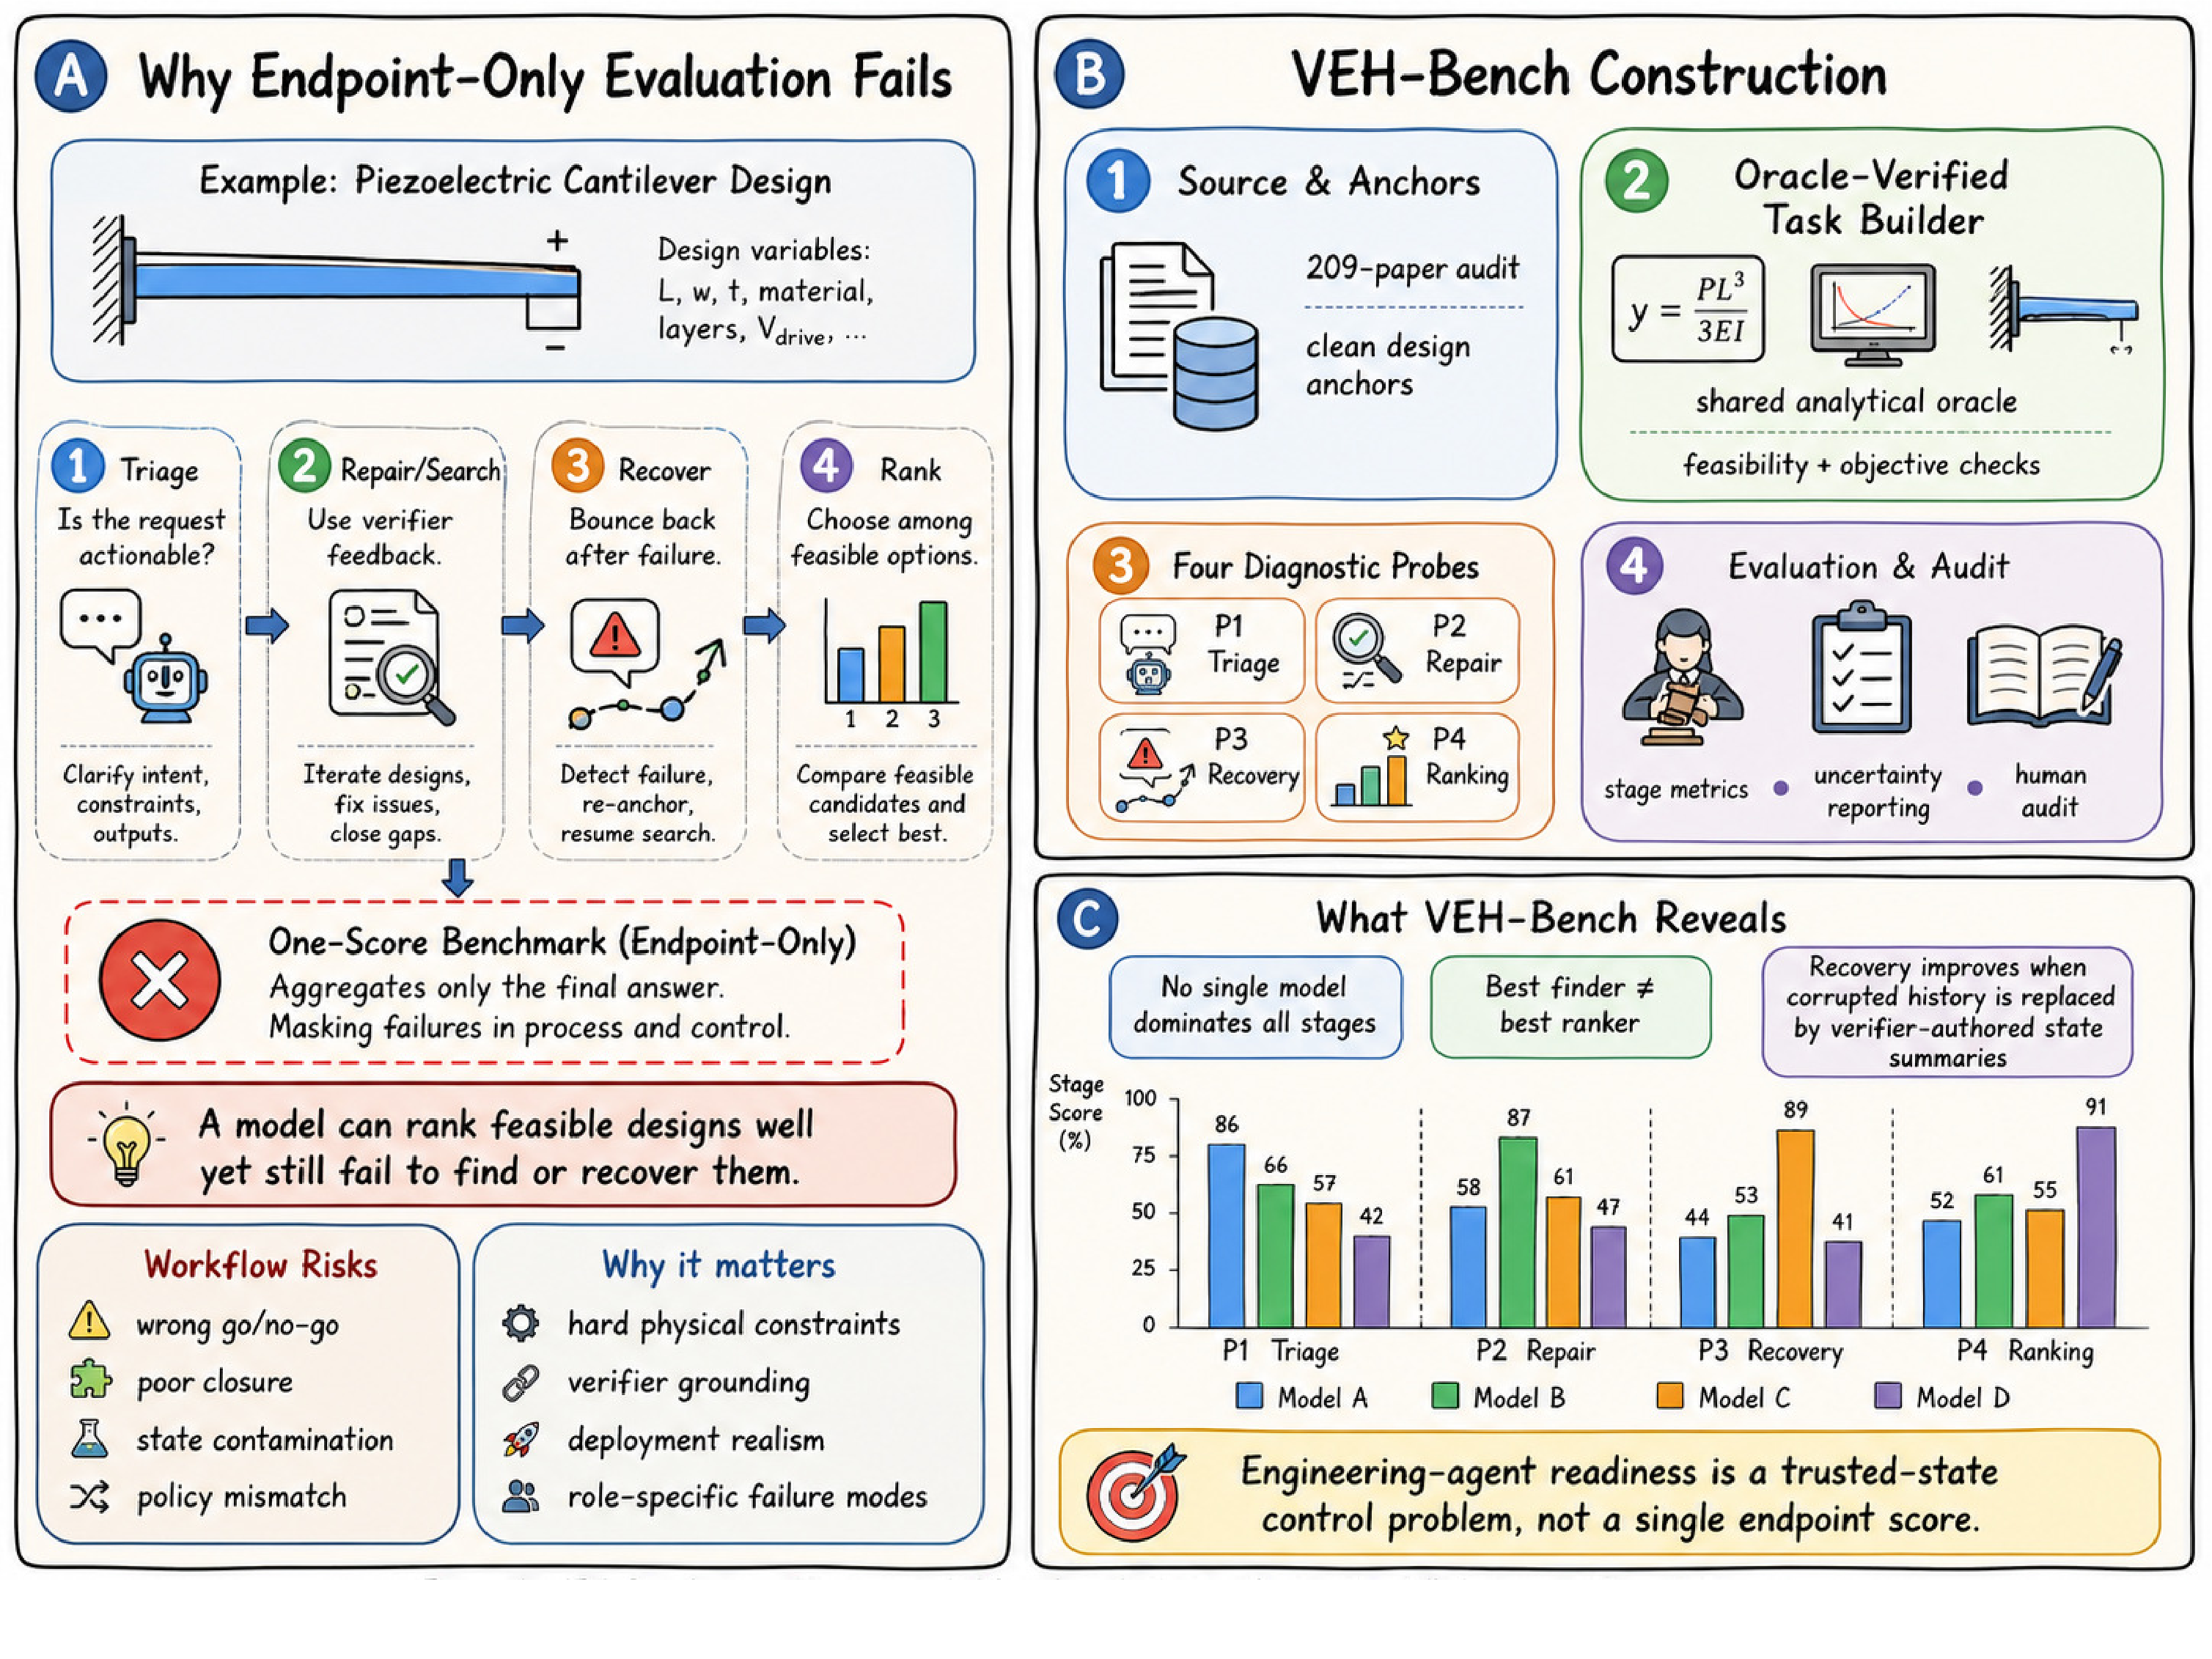
\includegraphics[width=\linewidth]{figures/main/running_example.pdf}
\caption{DiagBench overview. Endpoint-only evaluation masks where engineering agents fail; VEH-Bench turns source-grounded anchors into oracle-verified P1--P4 probes and reports stage-local failures rather than a single endpoint score.}
\label{fig:running_example}
\end{figure*}

Three design challenges follow. First, physical validity must be externally adjudicated: once feasibility is negotiated only inside language, a wrong trajectory can become contaminated evidence. Second, the benchmark must decompose the workflow rather than merely make one long task harder, because a harder repair task still does not test triage, recovery, or policy-conditioned selection. Third, the benchmark must show that non-monotonic rankings are structural rather than noise; otherwise stage decomposition would be redundant.

DiagBench addresses these challenges with a verifier-grounded benchmark for engineering design agents. The current VEH instantiation contains 763 manifest-backed tasks derived from a 209-paper extraction audit, 52 cleaned structure-review anchors, DOI-disjoint optimizer-facing splits for P2--P4, and a shared analytical oracle. The four probes correspond to four trusted-state boundaries: P1 tests credible triage before search, P2 tests constrained repair under verifier feedback, P3 tests recovery after a corrupted trajectory, and P4 tests policy-conditioned ranking among feasible candidates. Figure~\ref{fig:running_example} gives the motivation and benchmark overview; Figure~\ref{fig:workflow} summarizes the full workflow design.

Our contributions are:
\begin{itemize}[leftmargin=5mm,itemsep=1mm,topsep=1mm]
    \item We propose a workflow-structured evaluation framework that separates four trusted-state boundaries and interprets stage dissociation through response-control prior-boundary mismatch (Sections~\ref{sec:method} and~\ref{sec:experiments}).
    \item We instantiate the framework as a 763-task VEH benchmark with manifest-backed provenance, a shared analytical oracle, and a documented construction path from extraction audit to released task banks (Section~\ref{sec:method}; Appendix).
    \item Across 12 complete model runs with explicit run-mode tags, we show that no model dominates all four stages; log-derived profile indicators strongly track stage outcomes, including action prior to P1 ($\rho=0.97$), edit style to P2 ($\rho=0.84$), and preference execution to P4 ($\rho=0.77$) (Section~\ref{sec:experiments}).
    \item We provide mechanism evidence: a 36-task P3 state-summary intervention improves recovery by 13.2 points and cuts cascade by 18.6 points, while a matched isomorphic probe shows a 26--61 point gap between feasible-set selection and construction (Section~\ref{sec:experiments}).
    \item We add a hardened closed-form circuit audit showing that the P1--P4 diagnostic framework transfers to a second engineering domain, while model rankings remain boundary-specific rather than globally monotonic (Section~\ref{sec:experiments}; Appendix).
\end{itemize}

\section{Benchmark Design}
\label{sec:method}

\subsection{Design Goals}

DiagBench is a verifier-grounded evaluation framework for engineering design agents, instantiated here on VEH design. The goal is not to create a larger endpoint leaderboard, but to make four load-bearing engineering decisions separately measurable under the same physical oracle. We use four design goals:
\begin{itemize}[leftmargin=5mm,itemsep=1mm,topsep=1mm]
    \item \textbf{Auditable validity:} physical feasibility and objective values must be decided by an external analytical oracle, not by language-model consensus.
    \item \textbf{Stage-specific diagnostics:} each decision boundary should have its own action space, trusted state, and headline metric.
    \item \textbf{Path-dependence visibility:} recovery from corrupted state should remain separate from repair from a clean initial design.
    \item \textbf{Policy visibility:} final selection should test whether the model follows an explicit policy among feasible candidates, not only whether it can generate a design.
\end{itemize}

\begin{figure*}[t]
\centering
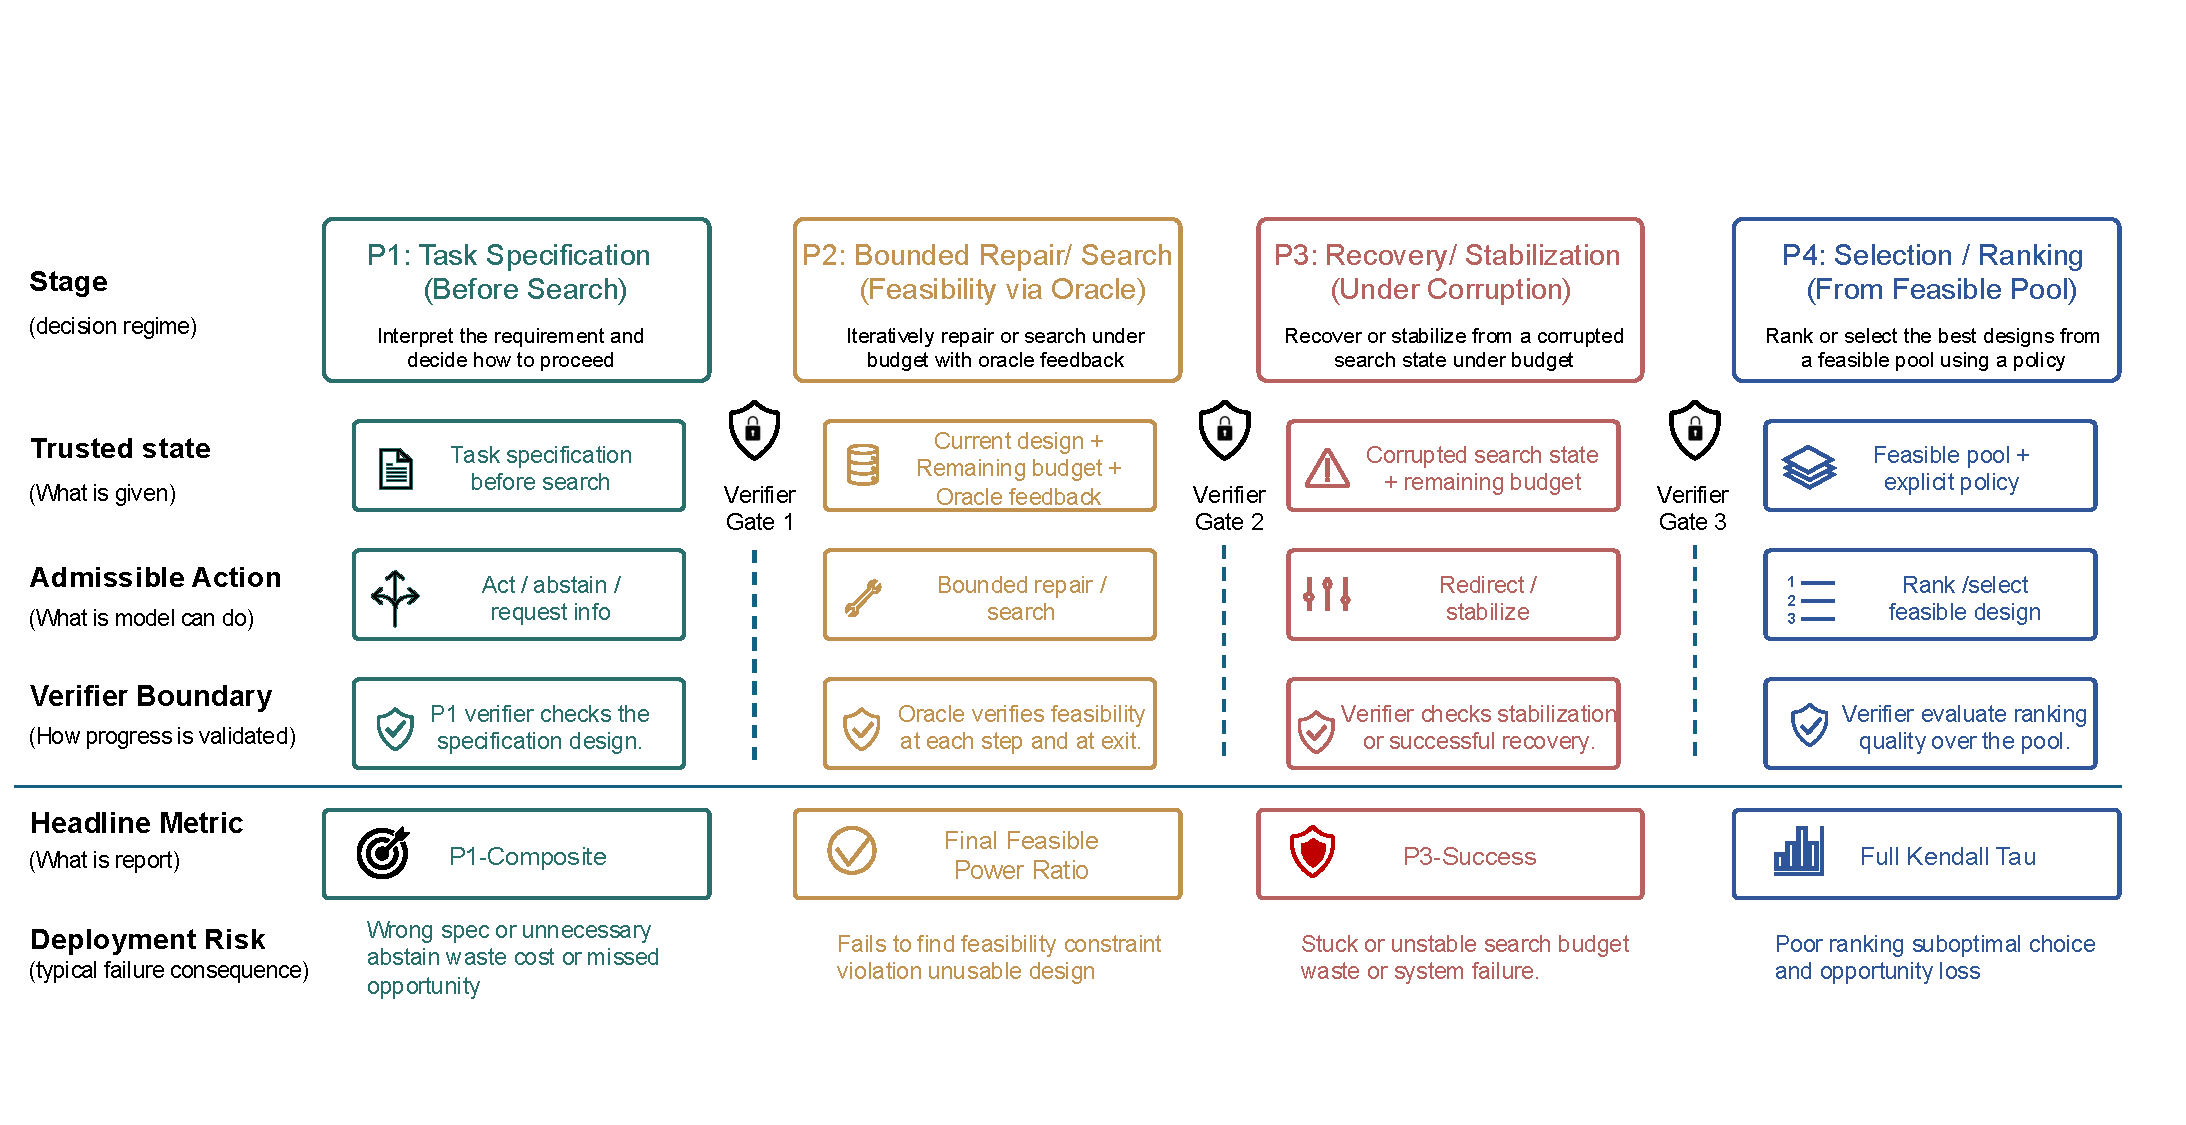
\includegraphics[width=\linewidth]{figures/main/workflow_diagram.pdf}
\caption{DiagBench as a workflow-structured benchmark. Each stage changes the trusted state, the permitted model action, and the headline metric, so endpoint-only evaluation cannot localize which control boundary failed.}
\label{fig:workflow}
\end{figure*}

\textbf{Running example.} A single VEH brief asks for a piezoelectric cantilever resonating at 50 Hz and delivering at least 15\,\textmu W under 0.5\,g excitation. DiagBench turns it into four questions. \textit{P1:} before search, should the agent propose a design, declare infeasibility, or request missing material information? \textit{P2:} from a seed design, can it iteratively repair frequency, power, stress, and displacement violations under oracle feedback? \textit{P3:} after a corrupted history has already moved in a harmful direction, can it reset the trusted state and recover? \textit{P4:} given five oracle-feasible candidates, can it rank them under a declared policy such as ``prioritize output power, then stress margin''? The physical object is shared; the trusted-state boundary is different.

\subsection{Probe Inventory}

\begin{table*}[t]
\caption{DiagBench inventory for the current VEH benchmark. Each probe corresponds to a different workflow boundary and therefore reports a different headline metric.}
\label{tab:inventory}
\centering
\small
\setlength{\tabcolsep}{4pt}
\renewcommand{\arraystretch}{1.08}
\begin{tabular}{lp{30mm}cp{36mm}p{33mm}}
\toprule
Probe & Workflow role & Tasks & Model action & Headline metric \\
\midrule
P1 & Credible triage & 240 & act, abstain, or request information & P1-Composite \\
P2 & Constrained repair/search & 208 & iterative verifier-guided edit & Final feasible power ratio \\
P3 & Post-trap recovery & 156 & reset or stabilize corrupted state & P3-Success \\
P4 & Policy-conditioned ranking & 159 & rank five feasible candidates & Full Kendall Tau \\
\bottomrule
\end{tabular}
\end{table*}

Table~\ref{tab:inventory} gives the main benchmark structure. P1 is a matched certification stress stage: it uses vetted anchor contexts rendered through subtype-balanced templates and is not claimed as a source-disjoint literature holdout. P2--P4 are optimizer-facing stages with DOI-disjoint source-anchor boundaries inherited from the cleaned VEH extraction pipeline. This distinction matters: cross-stage comparisons in this paper are stage-level comparisons under a shared verifier, not claims that all probes instantiate identical split semantics.

\textbf{P1: credible triage.} The model must output exactly one action: \texttt{propose\_design}, \texttt{declare\_infeasible}, or \texttt{request\_missing\_info}. The headline P1-Composite balances macro-F1, acceptance credibility, missing-information discipline, infeasibility discipline, and subtype F1, so raw accuracy alone cannot hide an over-act or over-refuse prior.

\textbf{P2: constrained repair/search.} The model iteratively edits VEH design variables under bounded query budget and oracle feedback. The headline final feasible power ratio rewards both reaching feasibility and preserving utility; first-step feasibility is diagnostic rather than primary.

\textbf{P3: post-trap recovery.} The model starts from a misleading search history that has already moved the design in a harmful direction. P3 separates trap escape, cascade avoidance, and final recovered feasibility; the headline is P3-Success.

\textbf{P4: policy-conditioned ranking.} The model ranks a pool of five oracle-feasible designs under an explicit policy. Full-bank Kendall Tau is the headline, while exact match, top-$k$ agreement, Pareto diagnostics, and BARS audit different ranking failure modes.

\subsection{Construction Pipeline and Oracle Boundary}

\begin{figure*}[t]
\centering
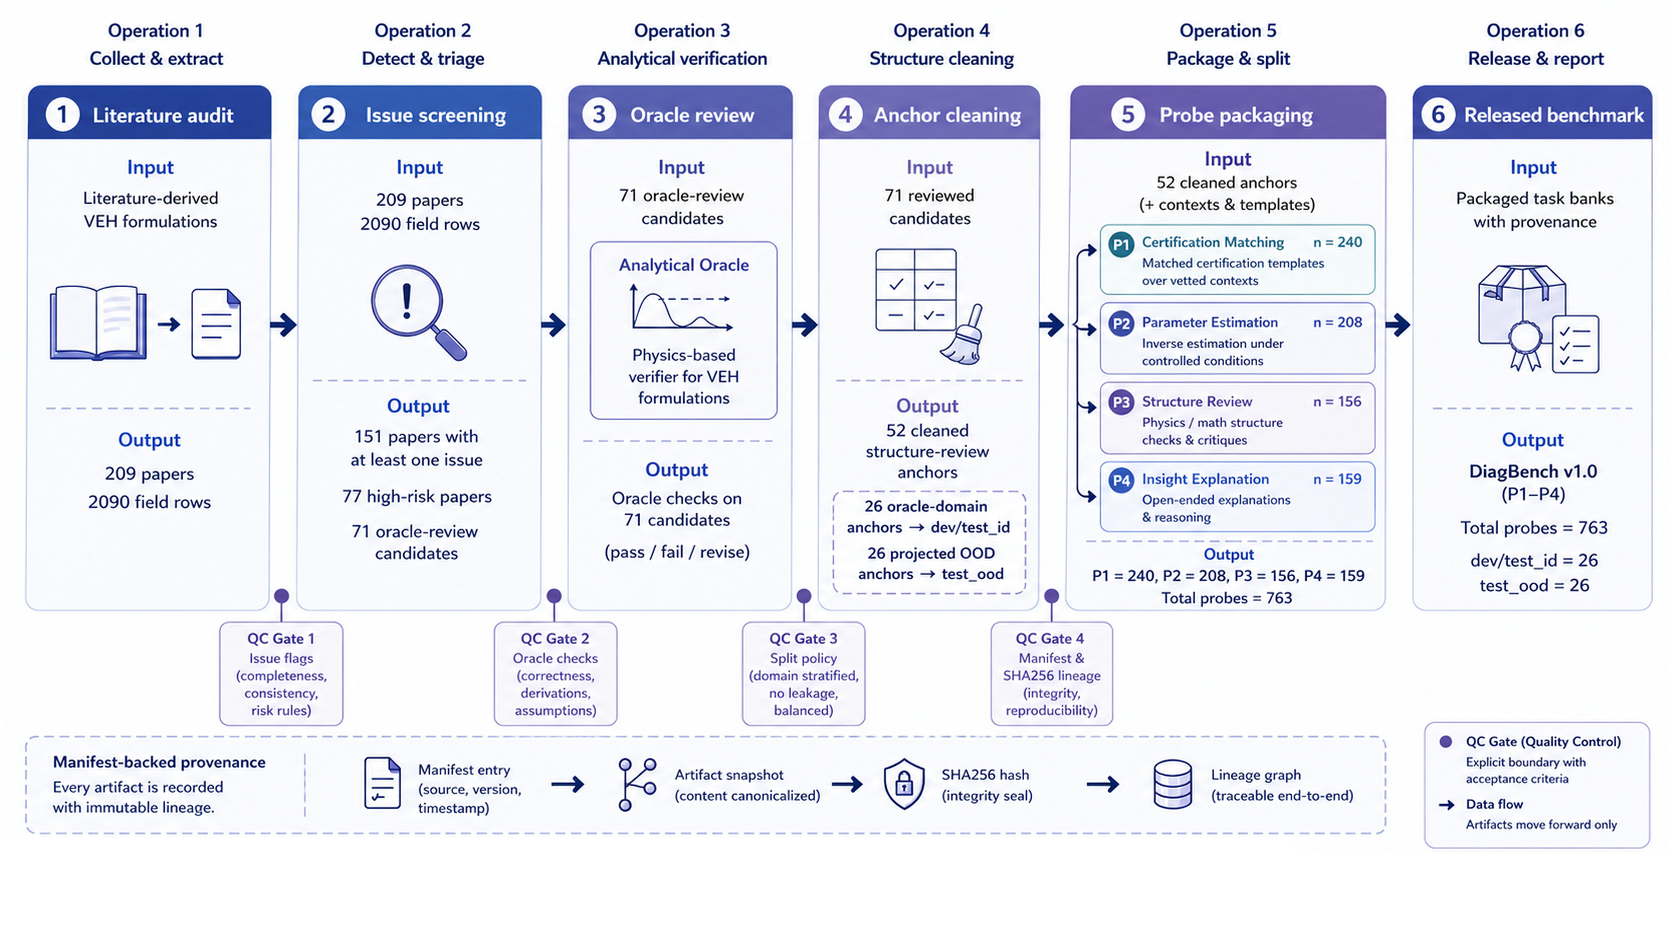
\includegraphics[width=\linewidth]{figures/main/construction_pipeline.pdf}
\caption{Benchmark construction pipeline. The figure summarizes source extraction, verifier review, QC gates, probe packaging, and manifest-backed release.}
\label{fig:construction_pipeline}
\end{figure*}

Figure~\ref{fig:construction_pipeline} summarizes the construction path. The upstream audit covers 209 papers and 2090 extracted field rows, flags high-risk extraction issues, and reduces the corpus to 71 oracle-review cantilever candidates. The current P2 backbone admits 52 cleaned structure-review anchors: 26 oracle-domain anchors routed into DOI-disjoint \texttt{dev}/\texttt{test\_id} splits and 26 projected out-of-domain-kept anchors routed to \texttt{test\_ood}. P3 and P4 inherit this optimizer-facing boundary. Eight unit-suspect papers remain explicitly flagged rather than silently rewritten. Full construction counts, split provenance, and intervention-subset sampling appear in Appendix Tables~\ref{tab:appendix_construction_audit},~\ref{tab:appendix_p3_subset_provenance}, and~\ref{tab:appendix_p3_intervention_delta_ci}.

The oracle boundary is fixed across probes. Each task specifies design variables, bounds, objectives, budgets, and any exposed history. Each proposal is parsed into a JSON action and passed to an analytical verifier, which returns feasibility, active violations, boundary-state labels, and objective information. Physical validity therefore remains external to the model. P2 may stop on feasible closure; P3 preserves the recovery trace so escape, late cascade, and dead-budget behavior remain observable.

The P3 intervention changes only the prompt-facing state representation. In raw-history mode, the model sees the corrupted trajectory. In \texttt{state\_summary} mode, it sees a deterministic verifier-authored summary of trusted fields: latest proposal, active violations, best-so-far feasible design, trend information, and remaining budget. The evaluator, stored trajectory, and oracle are unchanged. This makes the intervention a protocol audit of state isolation rather than a new benchmark variant.

\subsection{Artifact Availability}

The release artifact mirrors the benchmark claims: P1--P4 JSONL task banks, manifests, oracle and evaluator code, generation scripts, admission and split reports, and per-model JSONL logs. Contamination resistance is scoped to DOI/title deduplication, DOI-disjoint source-anchor separation for P2--P4, manifest-level lineage, and no duplicate task ids. We do not claim web-scale pretraining decontamination or model-specific near-duplicate removal. All artifacts are released under CC-BY-4.0 for data and MIT for code, with a Croissant metadata record documenting task schema, split policy, and intended use as an engineering-agent diagnostic benchmark. The benchmark is not intended for production safety certification or as a standalone engineering solver. A frozen anonymous release is available at the URL in the submission; maintenance will follow the DiagBench repository with versioned task banks and per-release manifest hashes.

\section{Empirical Findings}
\label{sec:experiments}

\subsection{Setup}

We evaluate 12 complete P1--P4 model runs on the 763-task VEH benchmark: gpt-5.4, \texttt{qwen3.6-plus}, deepseek-v3, claude-4.6-sonnet, qwen3-max, deepseek-r1, gemini-3.1-pro-preview, \texttt{o4-mini}, \texttt{llama-3.3-70b}, deepseek-v4-pro, mimo-v2.5-pro, and hunyuan-hy3-preview. Here \(n=12\) denotes model-level observations with all four probes complete, not a development split. The headline metrics are P1-Composite, P2 final feasible power ratio, P3-Success, and P4 full-bank Kendall Tau. Calibration references, split-resolved tables, uncertainty intervals, metric definitions, prompt templates, and the run-mode audit are in the appendix.

\subsection{Stage Dissociation: Engineering Ability Is Not One Scalar}

\begin{table*}[t]
\caption{Twelve-model P1--P4 headline results on the 763-task VEH benchmark. \texttt{Think} marks whether this run used reasoning/thinking mode; detailed run-mode evidence is in Appendix Table~\ref{tab:appendix_reasoning_grouping}.}
\label{tab:main_results}
\centering
\scriptsize
\setlength{\tabcolsep}{4pt}
\renewcommand{\arraystretch}{1.08}
\begin{tabular}{llcccc}
\toprule
Model & Think & P1 Comp. & P2 Ratio & P3 Succ. & P4 Tau \\
\midrule
qwen3-max & No & \textbf{0.574} & 0.1955 & 30.1 & 0.835 \\
gemini-3.1-pro-preview & Yes & 0.549 & \textbf{0.3904} & 37.2 & 0.824 \\
\texttt{o4-mini} & Yes & 0.518 & 0.1551 & 26.3 & 0.780 \\
deepseek-r1 & Yes & 0.504 & 0.2413 & 42.9 & 0.833 \\
gpt-5.4 & No & 0.428 & 0.1329 & 42.3 & \textbf{0.887} \\
hunyuan-hy3-preview & Yes & 0.425 & 0.1609 & \textbf{47.4} & 0.839 \\
deepseek-v3 & No & 0.369 & 0.1565 & 35.3 & 0.860 \\
\texttt{llama-3.3-70b} & No & 0.361 & 0.1197 & 3.2 & 0.714 \\
mimo-v2.5-pro & No & 0.317 & 0.1073 & 45.5 & 0.843 \\
\texttt{qwen3.6-plus} & No & 0.306 & 0.2063 & 27.6 & 0.877 \\
deepseek-v4-pro & No & 0.306 & 0.1294 & 28.8 & 0.794 \\
claude-4.6-sonnet & No & 0.207 & 0.2394 & 16.0 & 0.840 \\
\bottomrule
\end{tabular}
\end{table*}

Table~\ref{tab:main_results} is the central result. P1 is P1-Composite, P2 is final feasible power ratio, P3 is recovery success, and P4 is full-bank Kendall Tau; detailed run-mode evidence is in Appendix Table~\ref{tab:appendix_reasoning_grouping}. No model leads more than one headline stage: qwen3-max leads P1, gemini-3.1-pro-preview leads P2, hunyuan-hy3-preview leads P3, and gpt-5.4 leads P4. The strongest reversal is gemini-3.1-pro-preview versus gpt-5.4. gemini-3.1-pro-preview is the best feasible-set seeker in P2 but weak on P4 ranking; gpt-5.4 is the best policy-conditioned ranker but weak on P2 search. If engineering ability were one scalar, this pattern should be rare.

The within-stage diagnostics sharpen the same point. \textbf{P1 finding:} credible triage is not raw accuracy; qwen3-max wins the composite through balanced action discipline, while models with acceptable raw accuracy collapse once missing-information and infeasibility discipline are scored. \textbf{P2 finding:} start is not finish; gemini-3.1-pro-preview is not the best first-step model, but wins through sustained feasibility-preserving closure. \textbf{P3 finding:} escape is not recovery; gemini-3.1-pro-preview and claude-4.6-sonnet escape traps frequently but have very different cascade and final-success behavior. \textbf{P4 finding:} ranking is not one skill; full-order structure, exact endpoint agreement, and policy-active ranking separate. The full per-probe tables are in Appendix Tables~\ref{tab:appendix_p1_full}--\ref{tab:appendix_p4_full}.

\subsection{Response-Control Profiles: Why Dissociation Happens}

We next quantify response-control profiles directly from logs. The extractor uses P1 action distributions and false-action rates; P2 edit deltas, feasibility preservation, directed repair, and objective traces; P2/P3 verifier-feedback reduction consistency; P3 escape, cascade, dead-budget, and recovery-quality signals; and P4 full-ranking, BARS, exact-match, policy-sensitive-pair, parse, and Pareto diagnostics. The complete 12-model profile table is in Appendix Table~\ref{tab:profile_quantification}.

The intended diagonal relations are strong associations: action prior tracks P1-Composite (Spearman \(\rho=0.972\)), edit style tracks P2 ratio (\(\rho=0.839\)), and preference execution tracks P4 BARS (\(\rho=0.769\)) and full Tau (\(\rho=0.762\)). State trust is more structured: it does not monotonically track P3-Success because P3 separates escape, cascade, and conversion to feasibility, but it is negatively correlated with P2 ratio (\(\rho=-0.39\)) and P4 BARS (\(\rho=-0.55\)). A prior associated with strength at one boundary can therefore be associated with weakness at another.

\subsection{Ruling Out the Reasoning/Newness Explanation}

\begin{table*}[t]
\caption{Thinking mode versus response-control profile fit. Thinking-on runs help P3 on average but do not explain P1, P2, or P4 leaders; profile indicators localize the boundary-specific mechanism.}
\label{tab:reasoning_vs_profile}
\centering
\small
\setlength{\tabcolsep}{4.5pt}
\renewcommand{\arraystretch}{1.12}
\begin{tabular}{lccp{70mm}}
\toprule
Stage & Think & No-think & Profile-based interpretation \\
\midrule
P1 Composite & 0.499 & 0.359 & thinking-on runs are still not sufficient for triage; qwen3-max leads under a no-think provider-default call because action discipline is the measured dimension \\
P2 headline & 0.237 & 0.161 & gemini-3.1-pro-preview drives the think mean, but the operative boundary fit is bounded local edit style plus feedback obedience \\
P3 Success (\%) & 38.5 & 28.6 & largest group gap; corrupted-state recovery is where state skepticism and explicit replanning are most useful \\
P4 Full Tau & 0.819 & 0.831 & reversal; thinking mode does not guarantee policy-conditioned evaluator discipline \\
\bottomrule
\end{tabular}
\end{table*}

Table~\ref{tab:reasoning_vs_profile} rules out the shallow reading that DiagBench is only a reasoning-model leaderboard. Thinking-on runs help the corrupted-state boundary on average, but they do not determine the P1, P2, or P4 frontier. The same is true for recency: deepseek-v4-pro does not monotonically dominate deepseek-v3 or deepseek-r1. A more diagnostic account is boundary fit: P2 rewards bounded repair, P3 rewards state skepticism, and P4 rewards evaluator-role discipline.

\subsection{Mechanism Evidence: Four Validity Challenges, Four Responses}

We test four alternative explanations with matched audits: repair versus corrupted-state recovery, selection versus generation, LLM repair versus generic optimization, and structural profile mismatch versus prompt artifact. Each audit changes one part of the evaluation setup while keeping the relevant task boundary fixed.

\paragraph{Corrupted recovery is not clean repair.}
If P3 failure were only weak repair, replacing raw trajectory history with a verifier-authored state summary should not help systematically. If failure reflects corrupted-state entrapment, the intervention should reduce cascade and improve recovery. Figure~\ref{fig:mechanism_evidence} shows the expected pattern: \texttt{state\_summary} raises model-mean recovery from 50.0\% to 63.2\% and lowers cascade from 28.1\% to 9.5\%. Full numeric deltas and confidence intervals are in Appendix Table~\ref{tab:appendix_p3_intervention_delta_ci}.

\begin{figure*}[t]
\centering
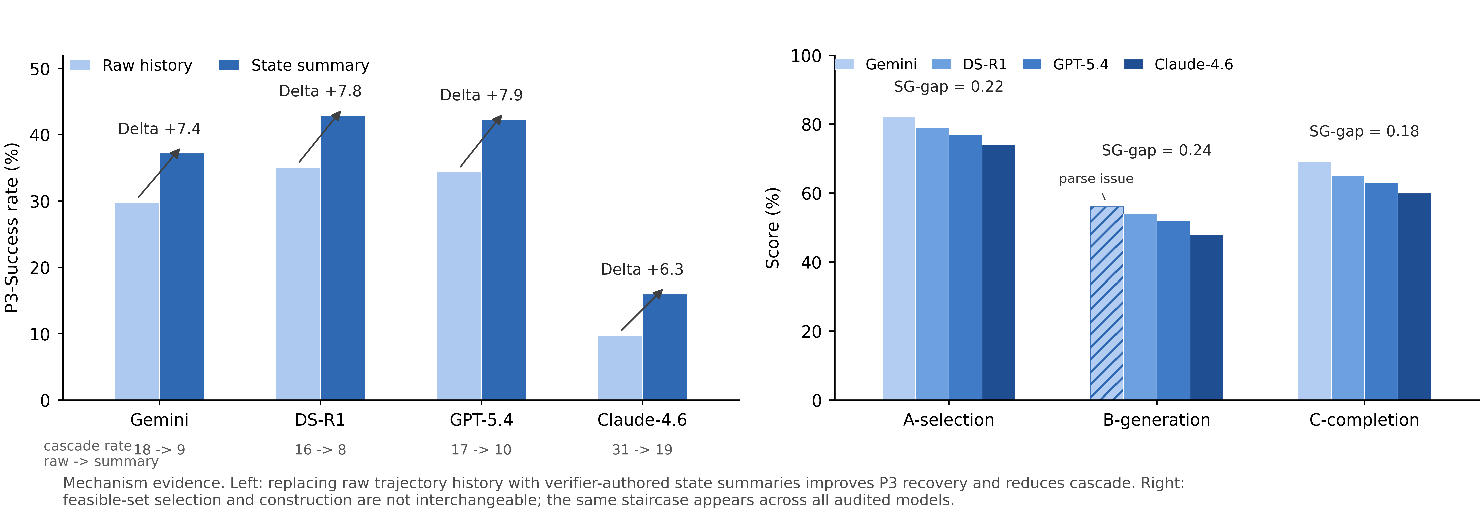
\includegraphics[width=\linewidth,trim=0 28bp 0 0,clip]{figures/main/selection_generation_gap.pdf}
\vspace{-5mm}
\caption{P3 intervention mechanism evidence. (A) Replacing raw trajectory history with a verifier-authored state summary improves recovery success for most models. (B) The same intervention reduces harmful cascade, showing that P3 is a corrupted-state boundary rather than ordinary clean repair. Full numeric results appear in Appendix Table~\ref{tab:appendix_p3_intervention_delta_ci}.}
\label{fig:mechanism_evidence}
\vspace{-3mm}
\end{figure*}

\paragraph{Selection is not generation.}
If P2 and P4 measured the same ability, selecting a feasible design should resemble generating it. The isomorphic audit holds the underlying feasible design fixed and changes only the model's role; it shows a 26--61 point gap between A-selection and B-generation. The gap is mostly capability rather than parsing for gpt-5.4, claude-4.6-sonnet, and \texttt{qwen3.6-plus}, supporting the claim that evaluative and generative priors are distinct. Full numeric results are in Appendix~\ref{sec:appendix_isomorphic}.

\paragraph{Repair is not generic optimization.}
If P2 reduced to numerical optimization, CMA-ES~\citep{hansen2023cma} should match LLM repair under the same 6-query oracle budget. It reaches 0.269 final feasible rate and 0.099 mean power ratio, below every frontier LLM; even at 40 queries it remains below gemini-3.1-pro-preview's P2 ratio. Full results appear in Appendix~\ref{sec:appendix_cmaes}, and the main conclusion is that P2 is not only an optimizer ceiling effect.

\paragraph{Profiles are not prompt artifacts.}
If the behavioral fingerprints above were shallow prompt artifacts, boundary-specific targeted prompts should repair known deficits. We test this with a pre-registered four-cell controlled-prompt experiment comparing default, neutral, targeted, wrong-boundary, and where applicable stacked prompts.

\begin{table*}[t]
\caption{Pre-registered controlled-prompt audit. Each cell reports the primary endpoint under the frozen prompt conditions; S+ denotes state-summary-plus for C2 only. Confidence intervals, secondary metrics, and parse rates are in Appendix~\ref{sec:tier3_full}.}
\label{tab:tier3_main}
\centering
\scriptsize
\setlength{\tabcolsep}{4pt}
\renewcommand{\arraystretch}{1.08}
\begin{tabularx}{\textwidth}{p{24mm}p{31mm}cccccY}
\toprule
Cell / endpoint & Model-stage & Default & Neutral & Targeted & Wrong & S+ & Readout \\
\midrule
C1 / P2 feasibility & gpt-5.4 & 0.150 & 0.175 & 0.150 & 0.075 & -- & targeted does not beat neutral \\
C2 / P3 success & claude-4.6-sonnet & 0.167 & \textbf{0.389} & 0.194 & 0.222 & 0.222 & neutral structure helps most \\
C3 / P4 Kendall $\tau$ & gemini-3.1-pro-preview & 0.692 & 0.692 & \textbf{0.708} & 0.700 & -- & one-task targeted gain \\
C4 / P1 accuracy & claude-4.6-sonnet & \textbf{0.650} & 0.617 & 0.567 & 0.633 & -- & targeted hurts format stability \\
C4 / P1 accuracy & gpt-5.4 & 0.433 & 0.400 & \textbf{0.467} & 0.400 & -- & small model-specific gain \\
\bottomrule
\end{tabularx}
\end{table*}

Table~\ref{tab:tier3_main} shows that targeted prompts do not consistently beat neutral structure. The strongest signal, claude-4.6-sonnet P3, reverses against the targeted prompt: neutral improves success most, while targeted and state-summary-plus remain low. This is consistent with durable prior-boundary mismatch rather than a signal that disappears under prompt rewriting; full condition-level results are in Appendix~\ref{sec:tier3_full}.

\subsection{Cross-Domain Construct Validity}

The mechanism audits address VEH-specific alternatives. The remaining question is whether the P1--P4 scaffold transfers when the physics changes. We instantiate a final circuit-design audit spanning closed-form RC filters, loaded dividers, LED current limiters, op-amp amplifiers, and linear regulators. It is not a circuit benchmark; it is a construct-validity check with a different oracle, different constraints, and different trap geometry.

\begin{table*}[t]
\caption{Circuit audit headline results. P1 is reported as P1-Composite; P2b is the final feasible objective score.}
\label{tab:circuit_pilot_headline}
\centering
\scriptsize
\setlength{\tabcolsep}{4pt}
\renewcommand{\arraystretch}{1.08}
\begin{tabular}{lccccccc}
\toprule
Model & P1 Comp. & P2 Feas. & P2b & P3 Succ. & P3 Casc. & P4 Tau & P4 BARS \\
\midrule
qwen3-max       & 0.971 & 0.906 & 0.494 & 0.778 & 0.471 & 0.608 & 0.710 \\
gemini-3.1-pro-preview  & \textbf{0.974} & \textbf{1.000} & \textbf{0.662} & \textbf{1.000} & \textbf{0.000} & 0.475 & 0.625 \\
gpt-5.4         & 0.923 & 0.875 & 0.457 & 0.778 & 0.176 & \textbf{0.625} & \textbf{0.722} \\
deepseek-r1     & \textbf{0.974} & 0.969 & 0.594 & 0.722 & \textbf{0.000} & 0.542 & 0.661 \\
hunyuan-hy3-preview     & 0.944 & 0.938 & 0.512 & 0.778 & 0.062 & 0.492 & 0.614 \\
claude-4.6-sonnet      & 0.932 & 0.906 & 0.487 & \textbf{1.000} & \textbf{0.000} & 0.608 & 0.707 \\
\midrule
Stage spread & 0.051 & 0.125 & 0.205 & 0.278 & 0.471 & 0.150 & 0.108 \\
\bottomrule
\end{tabular}
\end{table*}

Table~\ref{tab:circuit_pilot_headline} reproduces the main signature after replacing only P1/P2. No model dominates: gemini-3.1-pro-preview and deepseek-r1 tie the P1-Composite point estimate, gemini-3.1-pro-preview leads P2b, gemini-3.1-pro-preview and claude-4.6-sonnet retain the original P3 success lead, and gpt-5.4 retains the original P4 lead. The gpt-5.4 P4-over-P1/P2 reversal and gemini-3.1-pro-preview P2-over-P4 reversal both remain. The framework transfers; the rankings do not, which is what boundary-specific diagnosis predicts.

\section{Discussion}

\subsection{DiagBench as a Style-Boundary Compatibility Test}

DiagBench should be read as a style-boundary compatibility test, not as a global engineering leaderboard. Each probe changes the trusted state, model action, and failure consequence: P1 asks for entry discipline, P2 for verifier-feedback closure, P3 for contaminated-state reset, and P4 for policy-authorized selection. Frontier models arrive at these boundaries with different response-control priors. An over-act prior can help search persistence but hurt triage. A continuity-biased state prior can help ordinary feedback closure but harm corrupted-state recovery. An evaluator-role prior can help policy ranking while limiting generation-oriented search. The non-monotonic rankings are therefore not a nuisance; they are the measurement target.

This framing provides a compact account of the main apparent puzzles. Gemini leads P2 because its bounded local-edit style fits verifier-feedback repair, but the same generation-oriented style is less suited to P4 policy ranking. model_C leads P4 because it behaves like a disciplined evaluator, but that same profile does not produce strong P2 search closure. model_E gains most from the P3 state-summary intervention because its raw-history behavior shows strong continuity bias. Reasoning-style models shift P3 more than P1, P2, or P4 because state skepticism and explicit replanning are specifically useful at the contaminated-state boundary, while the other stages reward different priors.

\subsection{What the Evidence Establishes}

The strongest empirical claims are direct. First, the 12 complete model runs dissociate across P1--P4 under a shared verifier, and no model leads more than one headline stage. Second, replacing raw corrupted history with verifier-authored state summaries improves P3 recovery and reduces cascade on a frozen 36-task audit. Third, log-derived profile indicators are strongly stage-specific: action prior tracks P1, edit style tracks P2, and preference execution tracks P4. Fourth, the circuit audit reproduces the same diagnostic pattern in a second closed-form engineering domain.

Some claims remain interpretive rather than isolated causal conclusions. The five response-control dimensions are useful diagnostic indicators, but we do not claim they are complete or factorially separable. The P3 intervention changes the prompt-facing state representation, so its gain is consistent with verifier-authored state isolation but may also include compression, denoising, or formatting effects. The controlled-prompt audit (Section~\ref{sec:experiments}) tests whether Tier~1 behavioral fingerprints are causally upstream of performance; the null result supports the interpretation that these fingerprints reflect durable prior-boundary compatibility rather than prompt artifacts, but it does not isolate the exact cognitive mechanism. The circuit audit is a construct-validity check, not a full second benchmark. These boundaries matter: the paper's contribution is a verifier-grounded diagnostic framework and evidence that it exposes stable workflow dissociation, not a universal behavioral ontology.

\subsection{Implications for Engineering-Agent Systems}

The deployment implication is to route by boundary rather than by aggregate model rank. Search should be gated by a triage controller with balanced action discipline. Repair should use a model or prompt configuration whose edit style performs bounded, feasibility-preserving updates under oracle feedback. Recovery should not consume raw corrupted history as neutral context; continuity-biased models need verifier-authored state summaries or reset mechanisms. Final selection should be separated from generation because the best feasible-set seeker is not necessarily the best policy-conditioned evaluator. In short, engineering-agent systems should be verifier-gated, stage-routed, and policy-separated.

This also clarifies the role of classical optimization baselines. CMA-ES on the VEH P2 bank is useful calibration, but it does not replace the benchmark because DiagBench measures more than objective search. P1 tests actionability, P3 tests recovery after state contamination, and P4 tests policy-conditioned selection. Even inside P2, the key question is not only whether an optimizer can eventually improve utility, but whether an agent can close under a small oracle budget while preserving feasibility.

\subsection{Limits and Next Steps}

The main suite is anchored in VEH, and the hardened circuit audit is intentionally small. The analytical oracle makes the benchmark fast and auditable, but it narrows physical scope relative to high-fidelity simulation. P1 is a matched certification stress stage rather than a source-disjoint literature holdout. Some top-line gaps should be read with intervals rather than rhetoric, especially P3 and P4 near ties. The SG-gap audit currently covers four frontier models, and the P3 intervention covers a stratified subset rather than the full bank.

The next scaling step is not simply more VEH tasks. The portable object is the verifier-grounded decision scaffold: triage before search, bounded repair under feedback, recovery from corrupted state, and policy-conditioned selection among feasible candidates. Scaling this scaffold to thermal, structural, fluid, and circuit domains would test generality while preserving the same control boundaries. A second direction is factorial probing: vary feedback format, history length, policy explicitness, and verifier-authored summaries to isolate action prior, edit style, feedback obedience, state trust, and preference execution more cleanly than the current benchmark can.

\section{Related Work}
\label{sec:related_work}

DiagBench is closest to evaluation-first agent benchmarks that measure realistic workflows in executable environments. SWE-bench and LiveCodeBench evaluate software engineering ability~\citep{jimenez2024swebench,jain2024livecodebench}; MLE-bench extends this style to machine-learning engineering~\citep{chan2025mlebench}; AgentBench and $\tau$-bench emphasize interactive execution, tool use, and decision making~\citep{liu2024agentbench,yao2024taubench}. These benchmarks are valuable, but their primary readout is usually endpoint completion. DiagBench instead asks which trusted-state boundary failed: pre-search triage, verifier-guided repair, corrupted-state recovery, or policy-conditioned selection.

\begin{table*}[t]
\centering
\footnotesize
\setlength{\tabcolsep}{4.5pt}
\renewcommand{\arraystretch}{1.12}
\caption{Comparison with representative agent and engineering benchmarks. A filled dot denotes a dedicated evaluation target, a triangle denotes partial or indirect coverage, and an open circle denotes that the property is not a dedicated target.}
\label{tab:benchmark_scope_comparison}
\resizebox{\textwidth}{!}{%
\begin{tabular}{lcccccc}
\toprule
\textbf{Benchmark} &
\shortstack{\textbf{Executable}\\\textbf{verifier}} &
\shortstack{\textbf{Stage-specific}\\\textbf{metrics}} &
\shortstack{\textbf{Pre-search}\\\textbf{triage}} &
\shortstack{\textbf{Iterative}\\\textbf{repair}} &
\shortstack{\textbf{Corrupted-state}\\\textbf{recovery}} &
\shortstack{\textbf{Policy-conditioned}\\\textbf{ranking}} \\
\midrule
SWE-bench       & \(\bullet\) & \(\circ\) & \(\circ\) & \(\bullet\)   & \(\circ\) & \(\circ\) \\
LiveCodeBench   & \(\bullet\) & \(\circ\) & \(\circ\) & \(\bullet\)   & \(\circ\) & \(\circ\) \\
MLE-bench       & \(\bullet\) & \(\circ\) & \(\circ\) & \(\bullet\)   & \(\circ\) & \(\circ\) \\
AgentBench      & \(\bullet\) & \(\circ\) & \(\circ\) & \(\triangle\) & \(\circ\) & \(\circ\) \\
\(\tau\)-bench  & \(\bullet\) & \(\circ\) & \(\circ\) & \(\triangle\) & \(\circ\) & \(\circ\) \\
DiagBench       & \(\bullet\) & \(\bullet\) & \(\bullet\) & \(\bullet\) & \(\bullet\) & \(\bullet\) \\
\bottomrule
\end{tabular}%
}
\end{table*}

DiagBench is also adjacent to multi-agent orchestration systems such as AutoGen and MetaGPT~\citep{wu2023autogen,hong2024metagpt}, reward-model trajectory benchmarks such as Plan-RewardBench~\citep{wang2026planrewardbench}, and benchmark-design frameworks such as BIG-bench, HELM, WILDS, and How2Bench~\citep{srivastava2022bigbench,liang2023helm,koh2021wilds,cao2025how2bench}. The distinction is the oracle boundary: DiagBench evaluates the acting engineering agent under an external physical verifier, not an LLM judge or conversational closure loop. It also differs from reasoning-only narratives and black-box optimization suites such as COCO/BBOB~\citep{hansen2021coco}: explicit reasoning helps some stages, and numerical search is relevant to P2, but the benchmark target is broader--where the engineering workflow breaks, and which response-control prior mismatches the boundary.

\section{Conclusion}
\label{sec:conclusion}

DiagBench reframes engineering-agent evaluation around trusted-state boundaries rather than endpoint success. In a 763-task VEH benchmark with a shared analytical oracle, frontier models dissociate across credible triage, constrained repair, corrupted-state recovery, and policy-conditioned ranking; no model dominates all four stages.

The evidence is consistent with response-control prior-boundary compatibility. Action prior tracks P1, edit style tracks P2, preference execution tracks P4, and P3 separates escape, cascade, and recovery quality. A verifier-authored state-summary intervention improves P3 recovery and reduces cascade, while the isomorphic probe shows that feasible-set selection and construction are distinct behaviors. A hardened circuit audit supports the same P1--P4 diagnostic scaffold in a second closed-form engineering domain.

The system implication is practical: engineering agents should be verifier-gated, stage-routed, and policy-separated. A single endpoint score can hide the exact boundary where deployment fails; DiagBench is designed to make that failure localizable and auditable.


\clearpage
\bibliography{main}

\appendix
\newpage

\section*{\hspace{-4mm} \centering Appendix}
\vspace{3mm}

\section{Supplementary Roadmap}

The appendix supports the benchmark claims in the main paper rather than serving as a storage room for extra leaderboards. It is organized into four support blocks:
\begin{itemize}[leftmargin=5mm,itemsep=1mm,topsep=1mm]
    \item \textbf{Dataset and artifact audit:} construction provenance, artifact boundary, contamination scope, P3 intervention sampling, and release contents.
    \item \textbf{Metric and statistical definitions:} uncertainty intervals, calibration references, and formal definitions for every headline and diagnostic metric.
    \item \textbf{Full results and split checks:} complete P1--P4 tables, split-resolved tables, reasoning/thinking coverage, response-control profiles, and stage-gap diagnostics.
    \item \textbf{Mechanism and cross-domain audits:} extended related work/discussion, prompts, failure cases, selection--generation isomorphism, Tier~3 controlled-prompt results, CMA-ES, and the circuit audit.
\end{itemize}

\section{Construction Audit and Artifact Availability}

The current VEH suite is not a loose aggregation of prompts. Its optimizer-facing stages are traceable to a concrete literature-extraction and admission pipeline. The upstream extraction audit covers 209 papers and 2090 field rows, with 151 papers carrying at least one issue and 77 carrying a high-risk issue. From this audit, 71 cantilever candidates are forwarded to oracle review, and the current P2 backbone admits 52 cleaned structure-review anchors. The current benchmark then packages these anchors into split-specific task banks whose manifests store source tables, input manifest hashes, seeds, and artifact SHA256 values.

\Needspace{16\baselineskip}
\begin{center}
\captionof{table}{Construction audit for the current benchmark release. The table separates source scale, split policy, and release evidence so that the benchmark can be audited as a dataset rather than only as a set of scores.}
\label{tab:appendix_construction_audit}
\centering
\scriptsize
\setlength{\tabcolsep}{3pt}
\renewcommand{\arraystretch}{1.08}
\begin{tabularx}{\textwidth}{p{17mm}p{24mm}p{27mm}p{18mm}Y}
\toprule
Stage & Upstream source & Split policy & Final inventory & Audit detail \\
\midrule
P1 & vetted VEH anchor contexts rendered through eight certification templates & three matched partitions under three seeds; subtype-balanced and not DOI-disjoint & 240 = 80/80/80 & legacy \texttt{dev}/\texttt{test\_id}/\texttt{test\_ood} labels are bookkeeping only; partitions use 20/19/19 anchor contexts with pairwise overlap 19/19/18 \\
P2 & 52 cleaned structure-review anchors from the extraction audit & optimizer-facing splits are DOI-disjoint: 26 oracle-domain anchors feed \texttt{dev}/\texttt{test\_id}, 26 projected out-of-domain-kept anchors feed \texttt{test\_ood} & 208 = 64/40/104 & 8 unit-suspect papers retained with explicit flags; admission report records source-anchor counts and no dropped task ids \\
P3 & dual-constraint trap projection from P2 & inherits P2 optimizer-facing split boundary & 156 = 64/40/52 & manifests record source P2 task bank, BKF table, split manifest, and trap policy \\
P4 & policy-conditioned ranking pools derived from P2 BKF records & inherits P2 optimizer-facing split boundary & 159 = 93/36/30 & 53 realized base pools across the release; manifests record profile counts, top-1 distinctness, and source-task lineage for each pool \\
\bottomrule
\end{tabularx}
\end{center}

The release package is designed around these manifests and is available through the anonymous artifact page at \href{https://anonymous.4open.science/r/diagbench-734D/README.md}{anonymous.4open.science/r/diagbench-734D}. It contains the exact task JSONL files and manifests for P1--P4, the oracle and evaluator code, the task-generation scripts, the admission and split reports, and the per-model JSONL run logs used for the main and appendix tables. The intended artifact boundary is therefore the same as the paper boundary: each reported benchmark table should be traceable to a specific manifest-backed snapshot rather than to an undocumented local run.

Contamination resistance in the current release is deliberately scoped. It means DOI/title-hash deduplication in the upstream paper registry, DOI-disjoint source-anchor separation for P2--P4, manifest-level lineage tracking, and evaluation on post-fix noleak P1 runs only. It does \emph{not} mean that we claim web-scale near-duplicate search over model pretraining corpora or model-specific pretraining decontamination. P1 is intentionally outside the source-disjoint claim and should be read as a matched robustness stress stage rather than as a held-out generalization benchmark.

\section{P3 Intervention Provenance}

The P3 intervention in the main paper is intentionally not a rerun over the entire 156-task bank. It is a frozen protocol audit on a 36-task subset selected by stratified sampling over \texttt{split} $\times$ \texttt{source\_p2\_subtype}. The selection rule is: draw three tasks per observed stratum, then top up to 12 tasks per split from the remaining pool while preserving split balance. This keeps every observed family visible while preventing the intervention table from collapsing to a single split.

\begin{table*}[t]
\caption{Full-bank versus intervention-subset composition for P3. The 36-task intervention subset is stratified rather than ad hoc: every observed split/subtype family is retained, and the final subset is exactly balanced across splits.}
\label{tab:appendix_p3_subset_provenance}
\centering
\small
\begin{tabular}{lp{50mm}p{50mm}}
\toprule
Split & Full 156-task bank & 36-task intervention subset \\
\midrule
\texttt{dev} & 64 tasks: boundary\_binding 20, paper\_like 17, power\_tight 12, resonance\_tuned 15 & 12 tasks: 3 / 3 / 3 / 3 across the same four strata \\
\texttt{test\_id} & 40 tasks: boundary\_binding 10, paper\_like 4, power\_tight 15, resonance\_tuned 11 & 12 tasks: 3 / 3 / 3 / 3 across the same four strata \\
\texttt{test\_ood} & 52 tasks: projected\_boundary 18, projected\_resonance 34 & 12 tasks: projected\_boundary 3, projected\_resonance 9 after split-balanced top-up \\
\bottomrule
\end{tabular}
\end{table*}

\section{Statistical Validity}

Headline gaps should be paired with uncertainty rather than interpreted as isolated point estimates. For continuous aggregates such as P1-Composite, P2 final feasible power ratio, and P4 Kendall-style scores, we use nonparametric bootstrap intervals over task rows. For binary proportions such as P3-Success, we report Wilson intervals. Paired bootstrap deltas are used for the main near ties and for the P3 intervention audit so that uncertainty reflects within-task covariance rather than independent resampling.

\begin{table*}[t]
\caption{Headline uncertainty table for the four main probes.}
\label{tab:appendix_ci_table}
\centering
\scriptsize
\setlength{\tabcolsep}{3.5pt}
\renewcommand{\arraystretch}{1.08}
\begin{tabular}{lp{23mm}p{18mm}p{23mm}p{25mm}p{36mm}}
\toprule
Probe & Metric & Best & 95\% CI & Key delta & Note \\
\midrule
P1 & P1-Composite & 0.574 & [0.500, 0.641] & qwen3-max $-$ gemini-3.1-pro-preview: +0.025 [-0.078, 0.121] & not a trivial propose-bias win \\
P2 & feasible power ratio & 0.3904 & [0.3598, 0.4235] & gemini-3.1-pro-preview $-$ claude-4.6-sonnet: +0.1510 [0.1117, 0.1891] & separates closure from anchoring \\
P3 & P3-Success & 42.9\% & [35.4, 50.8]\% & R1 $-$ gpt-5.4: +0.6 pts [-7.1, 8.3] & near tie at the recovery frontier \\
P4 & Kendall Tau & 0.887 & [0.862, 0.911] & gpt-5.4 $-$ qwen3.6-plus: +0.013 [-0.024, 0.050] & calibrates ranking claims \\
\bottomrule
\end{tabular}
\end{table*}

\begin{table*}[t]
\caption{Near-tie paired tests that matter most to the main paper.}
\label{tab:appendix_near_ties}
\centering
\scriptsize
\setlength{\tabcolsep}{3pt}
\renewcommand{\arraystretch}{1.08}
\begin{tabularx}{\textwidth}{p{32mm}p{38mm}Y}
\toprule
Pair & Test object & Why this pair matters \\
\midrule
deepseek-r1 vs gpt-5.4 & P3-Success / RecoveryQuality & current recovery near tie; mechanism differs even if win disappears \\
gpt-5.4 vs qwen3.6-plus & P4 Full Tau / Exact & structural ranking versus endpoint preference matching \\
qwen3-max vs gemini-3.1-pro-preview & P1-Composite / P2 headline & certification-versus-closure split \\
\bottomrule
\end{tabularx}
\end{table*}

\begin{table*}[t]
\caption{P3 intervention numeric results. Delta columns report paired task-bootstrap 95\% intervals for \texttt{state\_summary} versus raw history.}
\label{tab:appendix_p3_intervention_delta_ci}
\centering
\scriptsize
\setlength{\tabcolsep}{4pt}
\renewcommand{\arraystretch}{1.08}
\begin{tabular}{lcccc}
\toprule
Model & Succ. raw/sum. & $\Delta$ success & Casc. raw/sum. & $\Delta$ cascade \\
\midrule
deepseek-r1 & 55.6 / 58.3 & +2.8 pts [-11.1, +16.7] & 30.3 / 8.7 & -21.6 pts [-37.5, -7.2] \\
gpt-5.4 & 63.9 / 63.9 & +0.0 pts [-13.9, +13.9] & 29.4 / 0.0 & -29.4 pts [-45.5, -14.7] \\
gemini-3.1-pro-preview & 50.0 / 66.7 & +16.7 pts [-2.8, +36.1] & 46.9 / 25.0 & -21.9 pts [-43.6, +0.5] \\
claude-4.6-sonnet & 30.6 / 63.9 & +33.3 pts [+16.7, +50.0] & 5.7 / 4.3 & -1.4 pts [-8.6, +4.4] \\
\midrule
Model mean & 50.0 / 63.2 & +13.2 pts [+4.9, +21.5] & 28.1 / 9.5 & -18.6 pts [-26.6, -10.6] \\
\bottomrule
\end{tabular}
\end{table*}

\clearpage
\section{Metric Definitions}
\label{sec:metric_formulas}

This section defines the metrics used in the main paper and appendix. All scores are computed from persisted JSONL logs by deterministic evaluator code; no metric uses human annotation or LLM-as-a-judge.

\subsection{P1: Credible Triage}

P1 is a one-shot three-action decision problem with gold labels in
\(\{\texttt{propose\_design}, \texttt{declare\_infeasible}, \texttt{request\_missing\_info}\}\).

\textbf{Accuracy and Macro-F1.} Accuracy is micro-averaged over all P1 tasks. Macro-F1 is the unweighted mean of the three action-level F1 scores:
\begin{equation}
\text{Macro-F1}
= \frac{1}{3}\sum_{c\in\mathcal{C}} F_{1,c},
\qquad
F_{1,c}=
\frac{2\,\mathrm{Prec}_c\,\mathrm{Rec}_c}
{\mathrm{Prec}_c+\mathrm{Rec}_c}.
\end{equation}
If \(\mathrm{Prec}_c+\mathrm{Rec}_c=0\), the corresponding \(F_{1,c}\) is defined as zero.

\textbf{Discipline scores.} Let \(A_r\), \(M_r\), and \(I_r\) denote recall for \texttt{propose\_design}, \texttt{request\_missing\_info}, and \texttt{declare\_infeasible}. Let \(A_s\), \(M_s\), and \(I_s\) denote the corresponding spurious-action rates on tasks whose gold label is not that action. Then:
\begin{align}
\mathrm{ACS} &= A_r(1-A_s),\\
\mathrm{MDS} &= M_r(1-M_s),\\
\mathrm{IDS} &= I_r(1-I_s).
\end{align}
ACS penalizes habitual proposing, MDS penalizes over-requesting information, and IDS penalizes over-refusal.

\textbf{P1-Composite.} The P1 headline metric is the weighted certification score used by the evaluator:
\begin{equation}
\begin{aligned}
\mathrm{P1Comp}={}&
0.40\,F1_{\mathrm{3class}}
+0.20\,\mathrm{ACS}
+0.15\,\mathrm{MDS} \\
&+0.15\,\mathrm{IDS}
+0.10\,F1_{\mathrm{subtype}} .
\end{aligned}
\end{equation}

\subsection{P2: Constrained Repair / Search}

For a P2 trajectory, let \(\mathbf{x}_t\) be the design at step \(t\), \(V(\mathbf{x}_t)\ge0\) the total normalized oracle violation, and \(T\) the final evaluated step.

\textbf{First and final feasibility.} P2a is the fraction of tasks where \(V(\mathbf{x}_1)=0\). Final feasible rate is the fraction where \(V(\mathbf{x}_T)=0\).

\textbf{P2b final feasible power ratio.} For VEH tasks, the headline metric is:
\begin{equation}
\begin{aligned}
\mathrm{P2b}
= \frac{1}{N_{\mathrm{P2}}}\sum_{i=1}^{N_{\mathrm{P2}}}
&\mathbf{1}\!\left[V(\mathbf{x}^{(i)}_T)=0\right] \\
&\cdot
\frac{P_{\mathrm{out}}(\mathbf{x}^{(i)}_T)}
{P_{\mathrm{out}}(\mathbf{x}^{(i)}_{\mathrm{BKF}})} .
\end{aligned}
\end{equation}
The circuit audit uses the analogous final feasible objective score returned by the circuit oracle.

\textbf{Conditional objective ratio.}
\begin{equation}
\mathrm{CondObj} =
\frac{
\sum_{i:\,V(\mathbf{x}^{(i)}_T)=0}
\mathrm{obj}(\mathbf{x}^{(i)}_T)}
{|\{i: V(\mathbf{x}^{(i)}_T)=0\}|}.
\end{equation}

\textbf{Trajectory diagnostics.} Violation reduction consistency is the fraction of transitions with \(V(\mathbf{x}_{t+1})\le V(\mathbf{x}_t)-10^{-6}\). Directed repair rate is the fraction of violated-constraint updates that move the relevant oracle metric in the feedback-implied direction. Feasibility preservation is the fraction of feasible-to-feasible transitions. Mean log edit delta is:
\begin{equation}
\delta_{\mathrm{edit}}
=
\frac{1}{|\mathcal{D}|}\sum_{d\in\mathcal{D}}
\frac{\left|\log(x_{t+1,d}/x_{t,d})\right|}
{\log(x_d^{\max}/x_d^{\min})}.
\end{equation}
Over-edit and no-op rates threshold this quantity in the corresponding evaluator.

\subsection{P3: Post-Trap Recovery}

P3 starts from a corrupted trajectory state. Escape rate is the fraction of tasks where at least one step reduces violation relative to the trapped state. Cascade rate is the fraction of escaped tasks where a new structurally coupled violation appears after the escape move. Dead-budget rate is the fraction of tasks with no meaningful post-trap design change.

\textbf{P3-Success and recovery quality.}
\begin{equation}
\mathrm{P3Success}
= \frac{1}{N_{\mathrm{P3}}}
\sum_i \mathbf{1}\!\left[V(\mathbf{x}^{(i)}_T)=0\right].
\end{equation}
\begin{equation}
\mathrm{RecoveryQuality}
=
\frac{
\sum_{i:\,V(\mathbf{x}^{(i)}_T)=0}
\mathrm{obj}(\mathbf{x}^{(i)}_T)}
{|\{i: V(\mathbf{x}^{(i)}_T)=0\}|}.
\end{equation}
The raw-history versus state-summary delta is the paired task-level difference in P3-Success between the two prompt representations, reported with paired bootstrap intervals.

\subsection{P4: Policy-Conditioned Ranking}

Each P4 task contains five oracle-feasible candidates. Full Kendall \(\tau\) is Kendall \(\tau_b\) between the model ranking and oracle ranking. Exact match, top-1 accuracy, top-2 set accuracy, pairwise accuracy, and policy-flip accuracy are computed directly from the predicted order.

\textbf{BARS.} For the VEH P4-full bank, the headline BARS score is computed only on balanced-active rows:
\begin{equation}
\begin{aligned}
\mathrm{BARS}
= {}&0.55\,\tau_{\mathrm{BA}}
+0.25\,\mathrm{PairAcc}_{\mathrm{BA}} \\
&+0.20\,\mathrm{Exact}_{\mathrm{BA}},
\end{aligned}
\end{equation}
where BA denotes the balanced-active subset. For the circuit audit, the analogous ranking score uses scaled Kendall \((\tau+1)/2\), policy-flip accuracy, and exact match with the same weights.

\subsection{Response-Control Profile Scores}

Profile scores are log-derived diagnostics. For each dimension \(D\), the evaluator collects a fixed indicator set \(\mathcal{M}_D\), orients every indicator so higher is better, min-max scales it across the compared models, and averages:
\begin{equation}
\mathrm{Profile}_D(m)
=
\frac{1}{|\mathcal{M}_D|}
\sum_{q\in\mathcal{M}_D} z_q(m).
\end{equation}

\begin{center}
\captionof{table}{Indicators used for response-control profile extraction. All indicators are direction-normalized before averaging.}
\label{tab:appendix_profile_indicator_sets}
\scriptsize
\setlength{\tabcolsep}{4pt}
\renewcommand{\arraystretch}{1.08}
\begin{tabular}{lp{115mm}}
\toprule
Dimension & Indicators \\
\midrule
Action prior & P1 action-distribution alignment, macro-F1, missing recall, infeasible recall, propose precision, non-invalid rate \\
Edit style & P2 bounded-local-edit rate, feasibility preservation, directed repair, final feasible rate, non-destructive edit rate, protocol-valid rate \\
Feedback obedience & P2 violation reduction, P2 utility improvement, P2 best-so-far AUC, P3 violation reduction, P3 post-feedback feasible rate \\
State trust & P3 trap escape, explicit replan, escape quality, non-cascade rate, non-dead-budget rate, state-summary success gain, state-summary cascade reduction \\
Preference execution & P4 scaled full Tau, balanced-active BARS, balanced-active policy-sensitive pair accuracy, exact match, top-1 accuracy, non-Pareto-violation rate, non-parse-error rate \\
\bottomrule
\end{tabular}
\end{center}


\section{Calibration References}

Weak baselines are useful here because the benchmark is deliberately structured. For P1, the main concern is degenerate label-prior matching. For P2, the main concern is whether headline gains reflect true improvement beyond the literature-derived seed or only feasibility preservation. For P3, the relevant weak behavior is continuity with the corrupted state rather than explicit reset. For P4, the relevant floor is chance agreement with a five-item ordering.

\begin{table*}[t]
\caption{Calibration references corresponding to the main-text weak baselines. These are not competitors to the frontier roster; they anchor how much of each stage can be explained by trivial behavior.}
\label{tab:appendix_calibration}
\centering
\small
\begin{tabular}{lp{30mm}p{23mm}p{60mm}}
\toprule
Probe & Baseline reference & Score & Interpretation \\
\midrule
P1 & always-\texttt{propose\_design} on the dev split & 56.3\% accuracy, 0.240 macro-F1, 0.0 worst-action recall & a degenerate action prior can look superficially acceptable on raw accuracy, which is why P1-Composite and subtype-balanced reporting are necessary \\
P2 & anchor-fixed heuristic on the 208-task main bank & 100\% feasible coverage, 0.3065 mean power ratio & many frontier models fail to preserve even the trivial feasible anchor, while gemini-3.1-pro-preview is the only one to beat this heuristic on the headline utility ratio \\
P3 & last-state continuation / no-reset heuristic & 0\% explicit reset by construction; weak reference for escape, cascade, and recovery columns & the useful floor is not a single scalar success rate but the failure mode produced by trusting corrupted state; P3 therefore reports escape, cascade, dead-budget, and recovery jointly \\
P4 & uniform random permutation over five feasible candidates & $\mathbb{E}[\tau]=0$, exact 0.83\%, top-1 20\% & observed ranking scores are far above chance, so P4 is not a random-agreement artifact \\
\bottomrule
\end{tabular}
\end{table*}

\clearpage
\section{Full Leaderboard Tables}

The appendix carries the full all-model tables for each main probe so that the main-paper mechanism claims remain auditable. All four tables use the frozen 12-model complete roster; runs without complete P1--P4 coverage are excluded rather than imputed.

This block should be read as a diagnostic audit rather than four extra leaderboards. Read each table column-wise: the headline metric gives the rank, while the diagnostic columns explain why that rank occurred and what failure mode is being exposed. The formulas are collected in Appendix~\ref{sec:metric_formulas}; the paragraphs below summarize how each metric is computed, what behavior it is intended to reveal, and what conclusion follows from the observed table.

\begin{table*}[t]
\caption{Interpretive map for the appendix full-table block. Each table is tied to a benchmark claim rather than presented as metric inventory alone.}
\label{tab:appendix_fulltable_map}
\centering
\small
\begin{tabular}{lp{21mm}p{16mm}p{16mm}p{16mm}p{16mm}p{18mm}}
\toprule
Probe & Core columns & Diagnostic 1 & Diagnostic 2 & Diagnostic 3 & Diagnostic 4 & Primary mechanism claim served \\
\midrule
P1 & Acc / Macro-F1 / ACS / MDS / IDS / subtype F1 / composite & over-act prior & hard infeasibility misses & missing-info discipline & balanced selectivity & raw accuracy does not equal credible triage \\
P2 & P2a / P2b / final feasible rate / conditional ratio / Impr. (P2c) / queries & anchoring & closure & best-so-far improvement & query efficiency & start is not finish \\
P3 & success / recovery quality / trap escape / cascade / dead budget / explicit replan & no-escape failure & escaped-but-unrecovered & false recovery & post-escape quality & escape is not recovery \\
P4 & Full Tau / Exact / Top-1 / Top-2 / Pareto Tau / BARS & structural order & strict endpoint ranking & policy-active ranking & parse stability & structural ranking is not policy sensitivity \\
\bottomrule
\end{tabular}
\end{table*}

\Needspace{14\baselineskip}
\paragraph{P1 metrics and readout.}
P1 is a one-shot triage task. Accuracy counts exact agreement with the oracle label; macro-F1 averages the three action labels so that a model cannot score well by favoring the majority action. ACS, MDS, and IDS are discipline scores for \texttt{propose\_design}, \texttt{request\_missing\_info}, and \texttt{declare\_infeasible}; each multiplies recall by one minus the corresponding spurious-action rate. Subtype F1 checks whether performance holds across near-feasible, missing-info, and infeasible subtypes. The headline P1-Composite combines these terms, so it rewards balanced entry discipline rather than raw willingness to produce a design. The table shows why this is necessary: several models have similar raw accuracy, but qwen3-max and gemini-3.1-pro-preview separate because their discipline scores are more balanced, while claude-4.6-sonnet exposes over-refusal or action-mismatch behavior that accuracy alone would under-explain.

\begin{center}
\captionof{table}{P1 full table. Compact headers keep certification metrics readable.}
\label{tab:appendix_p1_full}
\scriptsize
\setlength{\tabcolsep}{3.5pt}
\renewcommand{\arraystretch}{1.08}
\begin{tabular}{llllllll}
\toprule
Model & Acc & F1 & ACS & MDS & IDS & Subtype F1 & Comp. \\
\midrule
qwen3-max & 65.4\% & 0.647 & 0.429 & 0.533 & 0.486 & 0.768 & 0.574 \\
gemini-3.1-pro-preview & 69.2\% & 0.636 & 0.430 & 0.667 & 0.218 & 0.762 & 0.549 \\
\texttt{o4-mini} & 70.0\% & 0.623 & 0.388 & 0.396 & 0.361 & 0.776 & 0.518 \\
deepseek-r1 & 66.2\% & 0.594 & 0.360 & 0.510 & 0.298 & 0.730 & 0.504 \\
gpt-5.4 & 43.3\% & 0.486 & 0.224 & 0.657 & 0.223 & 0.569 & 0.428 \\
hunyuan-hy3-preview & 66.2\% & 0.539 & 0.295 & 0.333 & 0.200 & 0.700 & 0.425 \\
deepseek-v3 & 64.6\% & 0.483 & 0.206 & 0.352 & 0.100 & 0.668 & 0.369 \\
\texttt{llama-3.3-70b} & 62.5\% & 0.467 & 0.242 & 0.200 & 0.192 & 0.669 & 0.361 \\
mimo-v2.5-pro & 61.7\% & 0.433 & 0.152 & 0.244 & 0.083 & 0.644 & 0.317 \\
\texttt{qwen3.6-plus} & 61.3\% & 0.422 & 0.143 & 0.200 & 0.100 & 0.641 & 0.306 \\
deepseek-v4-pro & 61.3\% & 0.422 & 0.143 & 0.200 & 0.100 & 0.641 & 0.306 \\
claude-4.6-sonnet & 57.5\% & 0.305 & 0.057 & 0.000 & 0.100 & 0.583 & 0.207 \\
\bottomrule
\end{tabular}
\end{center}

\noindent\textbf{Audit note.} The exact tie between \texttt{qwen3.6-plus} and deepseek-v4-pro is preserved from the frozen scoring snapshot rather than broken by post-hoc rounding or reranking. Exact vector ties are therefore treated as tied diagnostic rows, not as evidence for an ordering between the two models.

\noindent\textbf{Takeaway.} P1 separates credible entry control from raw action frequency: the strongest rows combine reasonable proposing with missing-information and infeasibility discipline, while weak rows expose over-refusal or over-action even when accuracy is not catastrophic.

\Needspace{14\baselineskip}
\paragraph{P2 metrics and readout.}
P2 is an iterative repair task under verifier feedback. P2a is first-step feasibility, which measures whether the first edit lands directly in a feasible region. P2b is the headline final feasible power ratio: the final design contributes only if it is feasible, and its output power is normalized by the benchmark-known feasible reference. Final feasibility separates closure from objective quality, conditional ratio reports quality only among successful repairs, improvement measures best-so-far utility gain, AUC summarizes trajectory quality across the budget, and queries records how many oracle calls were needed. The main conclusion is that search closure and utility are not the same: gemini-3.1-pro-preview dominates P2b because it combines high final feasibility with high feasible utility, while models with respectable first-step feasibility can still finish with low final ratio if their subsequent edits overfit one constraint or lose power.

\begin{center}
\captionof{table}{P2 full table. P2a is first-step feasibility; P2b is the headline final feasible power ratio.}
\label{tab:appendix_p2_full}
\scriptsize
\setlength{\tabcolsep}{3.5pt}
\renewcommand{\arraystretch}{1.08}
\begin{tabular}{llllllll}
\toprule
Model & P2a & P2b & Final feas. & Cond. ratio & Impr. & AUC & Queries \\
\midrule
gemini-3.1-pro-preview & 26.0\% & 0.3904 & 96.2\% & 0.4101 & 0.7902 & 0.3388 & 2.63 \\
deepseek-r1 & 29.8\% & 0.2413 & 67.8\% & 0.3585 & 0.7901 & 0.2999 & 3.47 \\
claude-4.6-sonnet & 13.0\% & 0.2394 & 62.5\% & 0.3891 & 0.7037 & 0.2797 & 4.41 \\
\texttt{qwen3.6-plus} & 30.8\% & 0.2063 & 61.1\% & 0.3432 & 0.6466 & 0.2880 & 3.87 \\
qwen3-max & 23.6\% & 0.1955 & 55.8\% & 0.3537 & 0.6649 & 0.2894 & 4.21 \\
hunyuan-hy3-preview & 2.4\% & 0.1609 & 48.6\% & 0.3380 & 0.8033 & 0.2480 & 4.79 \\
deepseek-v3 & 7.2\% & 0.1565 & 44.2\% & 0.3576 & 0.5907 & 0.2766 & 4.68 \\
\texttt{o4-mini} & 22.6\% & 0.1551 & 42.8\% & 0.3665 & 0.7571 & 0.3119 & 3.59 \\
gpt-5.4 & 7.2\% & 0.1329 & 36.1\% & 0.3841 & 0.6828 & 0.2708 & 4.75 \\
deepseek-v4-pro & 30.3\% & 0.1294 & 41.3\% & 0.3205 & 0.6167 & 0.2935 & 4.26 \\
\texttt{llama-3.3-70b} & 23.6\% & 0.1197 & 37.0\% & 0.3277 & 0.6673 & 0.2895 & 4.38 \\
mimo-v2.5-pro & 26.4\% & 0.1073 & 33.2\% & 0.3282 & 0.6714 & 0.3075 & 4.50 \\
\bottomrule
\end{tabular}
\end{center}

\noindent\textbf{Takeaway.} P2 is won by feasible closure plus useful final power, not by first-step feasibility alone; gemini-3.1-pro-preview's lead is therefore a repair-trajectory result rather than an anchoring artifact.

\Needspace{14\baselineskip}
\paragraph{P3 metrics and readout.}
P3 starts from a corrupted trajectory. Success is final feasibility at the end of the recovery budget; recovery quality reports the objective quality among successful recoveries; first feasible identifies whether a model ever reaches a feasible state early in the recovery trace. Escape measures whether the model moves away from the known trap, cascade records whether the escape introduces a new coupled violation, dead-budget marks trajectories with no meaningful recovery action, and replan counts explicit reset or replanning behavior. These columns show that P3 is not ordinary repair: claude-4.6-sonnet is the clearest diagnostic row, with 96.8\% escape but only 0.6\% first-feasible and 16.0\% final success. It often notices that the raw history is wrong, but it rarely stabilizes back into a feasible design. deepseek-r1 and gpt-5.4 combine high escape with better final recovery; hunyuan-hy3-preview and mimo-v2.5-pro lead success through different trade-offs in recovery quality and cascade control.

\begin{center}
\captionof{table}{P3 full table. Columns separate recovery success, escape, cascade, dead-budget, and replanning behavior.}
\label{tab:appendix_p3_full}
\scriptsize
\setlength{\tabcolsep}{3.5pt}
\renewcommand{\arraystretch}{1.08}
\begin{tabular}{llllllll}
\toprule
Model & Succ. & RecQ & First feas. & Escape & Cascade & Dead & Replan \\
\midrule
hunyuan-hy3-preview & 47.4\% & 0.4876 & 40.4\% & 77.6\% & 9.1\% & 25.3\% & 7.7\% \\
mimo-v2.5-pro & 45.5\% & 0.6263 & 41.0\% & 63.5\% & 4.0\% & 26.7\% & 17.9\% \\
deepseek-r1 & 42.9\% & 0.2708 & 22.4\% & 92.3\% & 26.4\% & 25.1\% & 26.3\% \\
gpt-5.4 & 42.3\% & 0.3723 & 26.3\% & 90.4\% & 21.3\% & 25.2\% & 6.4\% \\
gemini-3.1-pro-preview & 37.2\% & 0.3194 & 26.9\% & 92.3\% & 50.7\% & 25.8\% & 10.9\% \\
deepseek-v3 & 35.3\% & 0.2868 & 23.1\% & 82.7\% & 27.1\% & 27.6\% & 57.7\% \\
qwen3-max & 30.1\% & 0.2612 & 22.4\% & 85.9\% & 12.7\% & 25.7\% & 49.4\% \\
deepseek-v4-pro & 28.8\% & 0.1986 & 27.6\% & 90.4\% & 17.0\% & 24.3\% & 99.4\% \\
\texttt{qwen3.6-plus} & 27.6\% & 0.1453 & 12.8\% & 94.9\% & 23.0\% & 25.6\% & 0.6\% \\
\texttt{o4-mini} & 26.3\% & 0.1389 & 12.2\% & 69.2\% & 17.6\% & 26.6\% & 8.3\% \\
claude-4.6-sonnet & 16.0\% & 0.0960 & 0.6\% & 96.8\% & 5.3\% & 25.7\% & 0.0\% \\
\texttt{llama-3.3-70b} & 3.2\% & 0.0926 & 2.6\% & 34.6\% & 3.7\% & 14.3\% & 0.0\% \\
\bottomrule
\end{tabular}
\end{center}

\noindent\textbf{Takeaway.} P3 shows that escaping a corrupted trajectory is not the same as recovering: high escape with low success marks continuity or cascade failure, while successful recovery requires both reset and stabilization.

\Needspace{14\baselineskip}
\paragraph{P4 metrics and readout.}
P4 removes search from the problem: all candidates are oracle-feasible before the model ranks them. Full Kendall Tau measures global order agreement with the oracle policy ranking; exact match requires the entire five-item order to be correct; top-1 and top-2 set accuracy measure whether the highest-priority choices are preserved; Pareto Tau isolates ranking consistency on Pareto-relevant comparisons; BARS emphasizes balanced-active policy-sensitive rows; parse and violation rates record formatting failures and attempts to alter fixed candidates. The table shows that P4 is not reducible to one ranking statistic. gpt-5.4 leads Full Tau, qwen3.6-plus is strongest on exact match, and gemini-3.1-pro-preview has a high BARS despite lower Tau, indicating that policy execution has multiple sub-behaviors rather than a single scalar notion of ``ranking skill.''

\begin{center}
\captionof{table}{P4 full table. Compact notation keeps ranking, Pareto, and formatting diagnostics in one table.}
\label{tab:appendix_p4_full}
\scriptsize
\setlength{\tabcolsep}{3.5pt}
\renewcommand{\arraystretch}{1.08}
\begin{tabular}{llllllll}
\toprule
Model & Tau & Exact & Top1 & Top2 & Pareto & BARS & Parse / viol. \\
\midrule
gpt-5.4 & 0.887 & 57.2\% & 83.0\% & 81.1\% & 1.000 & 0.6258 & 0.0\% / 0.0\% \\
\texttt{qwen3.6-plus} & 0.877 & 66.3\% & 79.1\% & 83.4\% & 1.000 & 0.6912 & 0.0\% / 0.0\% \\
deepseek-v3 & 0.860 & 54.7\% & 77.4\% & 79.2\% & 0.984 & 0.5751 & 0.0\% / 0.8\% \\
mimo-v2.5-pro & 0.843 & 52.8\% & 72.3\% & 79.2\% & 0.993 & 0.6012 & 0.0\% / 0.3\% \\
claude-4.6-sonnet & 0.840 & 56.6\% & 72.3\% & 79.2\% & 1.000 & 0.6781 & 0.0\% / 0.0\% \\
hunyuan-hy3-preview & 0.839 & 50.9\% & 77.4\% & 79.9\% & 0.943 & 0.5610 & 0.0\% / 2.8\% \\
qwen3-max & 0.835 & 49.7\% & 78.0\% & 76.7\% & 0.983 & 0.5367 & 0.0\% / 0.8\% \\
deepseek-r1 & 0.833 & 56.0\% & 71.7\% & 76.7\% & 1.000 & 0.6835 & 0.0\% / 0.0\% \\
gemini-3.1-pro-preview & 0.824 & 54.1\% & 71.7\% & 78.6\% & 0.975 & 0.6988 & 1.3\% / 1.3\% \\
deepseek-v4-pro & 0.794 & 43.4\% & 60.4\% & 74.2\% & 0.977 & 0.5832 & 0.0\% / 1.2\% \\
\texttt{o4-mini} & 0.780 & 50.0\% & 60.0\% & 72.0\% & 1.000 & 0.5988 & 0.0\% / 0.0\% \\
\texttt{llama-3.3-70b} & 0.714 & 34.0\% & 54.1\% & 65.4\% & 0.959 & 0.5386 & 0.0\% / 2.0\% \\
\bottomrule
\end{tabular}
\end{center}

\noindent\textbf{Takeaway.} P4 ranking has multiple sub-behaviors: global order quality, exact endpoint order, top-choice preservation, and policy-sensitive BARS can diverge, which is why P4 is not reducible to one scalar preference score.

\section{Split-Resolved Tables}

This block checks that the main-paper claims are not driven by a single split. The P2 closure pattern and P4 non-monotonic ranking pattern remain visible across splits, while P3 contains genuine near ties that should be read with the confidence intervals in Appendix~\ref{tab:appendix_ci_table}. P1 uses matched partitions rather than DOI-disjoint source splits, so its split labels audit robustness rather than held-out generalization. The split-resolved and stage-gap tables use the frozen common-coverage split snapshot; later-added full-bank rows for hunyuan-hy3-preview, mimo-v2.5-pro, and deepseek-v4-pro are included in the main full tables but not imputed into split/stage-gap views. Exact split-invariant rows, such as \texttt{qwen3.6-plus} and claude-4.6-sonnet in P1, are retained as audit signals from the released snapshot. Each table reports the main stage headline plus one supporting diagnostic in a split-resolved view.

\begin{table*}[t]
\caption{Split and subtype reporting plan. The appendix presents split-resolved views as mechanism audits rather than as extra leaderboards.}
\label{tab:appendix_split_subtype_map}
\centering
\small
\begin{tabular}{lp{28mm}p{32mm}p{42mm}}
\toprule
Probe & Split-resolved view & Subtype families & Main claim audited \\
\midrule
P1 & matched-partition composite and diagnostics (legacy \texttt{dev}/\texttt{test\_id}/\texttt{test\_ood} labels) & infeasible-margin, infeasible-structural, missing-info families & certification robustness is not driven by one matched partition or blocker family \\
P2 & dev / test\_id / test\_ood headline and feasible rate & paper-like, resonance-tuned, power-tight, boundary-binding & closure dominates anchoring as the main search distinction \\
P3 & dev / test\_id / test\_ood success and recovery quality & trap families and cascade diagnostics & corrupted-state recovery is not reducible to nominal repair quality \\
P4 & dev / test\_id / test\_ood Full Tau and Exact & balanced, performance-first, reliability-first, BARS & structural ranking and policy-sensitive ranking remain partially separable \\
\bottomrule
\end{tabular}
\end{table*}

\begin{table*}[t]
\caption{P1 matched-partition table. Each cell reports P1-Composite and raw accuracy.}
\label{tab:appendix_p1_split}
\centering
\scriptsize
\setlength{\tabcolsep}{4pt}
\renewcommand{\arraystretch}{1.08}
\begin{tabular}{lccc}
\toprule
Model & dev & test\_id & test\_ood \\
\midrule
qwen3-max & 0.532 / 61.3\% & 0.622 / 70.0\% & 0.567 / 65.0\% \\
gemini-3.1-pro-preview & 0.545 / 70.0\% & 0.525 / 66.2\% & 0.578 / 71.2\% \\
\texttt{o4-mini} & 0.542 / 71.2\% & 0.509 / 70.0\% & 0.502 / 68.8\% \\
deepseek-r1 & 0.517 / 68.8\% & 0.512 / 66.2\% & 0.482 / 63.7\% \\
gpt-5.4 & 0.374 / 37.5\% & 0.469 / 47.5\% & 0.440 / 45.0\% \\
deepseek-v3 & 0.357 / 63.7\% & 0.385 / 65.0\% & 0.364 / 65.0\% \\
\texttt{llama-3.3-70b} & 0.362 / 61.3\% & 0.393 / 65.0\% & 0.328 / 61.3\% \\
\texttt{qwen3.6-plus} & 0.306 / 61.3\% & 0.306 / 61.3\% & 0.306 / 61.3\% \\
claude-4.6-sonnet & 0.207 / 57.5\% & 0.207 / 57.5\% & 0.207 / 57.5\% \\
\bottomrule
\end{tabular}
\end{table*}

\begin{table*}[t]
\caption{P2 split-resolved table. Each cell reports the final feasible power ratio and final feasible coverage.}
\label{tab:appendix_p2_split}
\centering
\scriptsize
\setlength{\tabcolsep}{4pt}
\renewcommand{\arraystretch}{1.08}
\begin{tabular}{lccc}
\toprule
Model & dev & test\_id & test\_ood \\
\midrule
gemini-3.1-pro-preview & 0.4017 / 98.4\% & 0.4324 / 90.0\% & 0.3672 / 97.1\% \\
deepseek-r1 & 0.2560 / 62.5\% & 0.3049 / 82.5\% & 0.2078 / 65.4\% \\
claude-4.6-sonnet & 0.2199 / 54.7\% & 0.3095 / 75.0\% & 0.2245 / 62.5\% \\
\texttt{qwen3.6-plus} & 0.2355 / 57.8\% & 0.2316 / 65.0\% & 0.1786 / 61.5\% \\
qwen3-max & 0.2182 / 50.0\% & 0.2486 / 60.0\% & 0.1612 / 57.7\% \\
deepseek-v3 & 0.2052 / 48.4\% & 0.1761 / 47.5\% & 0.1189 / 40.4\% \\
\texttt{o4-mini} & 0.1587 / 42.2\% & 0.1220 / 35.0\% & 0.1655 / 46.2\% \\
gpt-5.4 & 0.0991 / 26.6\% & 0.0541 / 12.5\% & 0.1841 / 51.0\% \\
\texttt{llama-3.3-70b} & 0.1781 / 43.8\% & 0.1046 / 32.5\% & 0.0896 / 34.6\% \\
\bottomrule
\end{tabular}
\end{table*}

\begin{table*}[t]
\caption{P3 split-resolved table. Each cell reports final recovered feasible rate and post-escape recovery quality.}
\label{tab:appendix_p3_split}
\centering
\scriptsize
\setlength{\tabcolsep}{4pt}
\renewcommand{\arraystretch}{1.08}
\begin{tabular}{lccc}
\toprule
Model & dev & test\_id & test\_ood \\
\midrule
deepseek-r1 & 45.3\% / 0.3103 & 37.5\% / 0.2105 & 44.2\% / 0.2708 \\
gpt-5.4 & 48.4\% / 0.4322 & 40.0\% / 0.3816 & 36.5\% / 0.2841 \\
gemini-3.1-pro-preview & 43.8\% / 0.3770 & 32.5\% / 0.2917 & 32.7\% / 0.2660 \\
deepseek-v3 & 42.2\% / 0.2368 & 27.5\% / 0.3571 & 32.7\% / 0.3068 \\
qwen3-max & 39.1\% / 0.3182 & 22.5\% / 0.1912 & 25.0\% / 0.2444 \\
\texttt{qwen3.6-plus} & 28.1\% / 0.1774 & 27.5\% / 0.1389 & 26.9\% / 0.1100 \\
\texttt{o4-mini} & 28.1\% / 0.1556 & 30.0\% / 0.1667 & 21.2\% / 0.0972 \\
claude-4.6-sonnet & 20.3\% / 0.1270 & 10.0\% / 0.0513 & 15.4\% / 0.0918 \\
\texttt{llama-3.3-70b} & 4.7\% / 0.1429 & 0.0\% / 0.0000 & 3.8\% / 0.1429 \\
\bottomrule
\end{tabular}
\end{table*}

\begin{table*}[t]
\caption{P4 split-resolved table. Each cell reports Full Tau and Exact.}
\label{tab:appendix_p4_split}
\centering
\scriptsize
\setlength{\tabcolsep}{4pt}
\renewcommand{\arraystretch}{1.08}
\begin{tabular}{lccc}
\toprule
Model & dev & test\_id & test\_ood \\
\midrule
gpt-5.4 & 0.886 / 53.8\% & 0.900 / 58.3\% & 0.873 / 66.7\% \\
\texttt{qwen3.6-plus} & 0.867 / 65.6\% & 0.870 / 57.5\% & 0.920 / 80.0\% \\
deepseek-v3 & 0.888 / 57.0\% & 0.783 / 47.2\% & 0.867 / 56.7\% \\
claude-4.6-sonnet & 0.832 / 59.1\% & 0.833 / 41.7\% & 0.873 / 66.7\% \\
qwen3-max & 0.832 / 49.5\% & 0.850 / 47.2\% & 0.827 / 53.3\% \\
deepseek-r1 & 0.834 / 57.0\% & 0.800 / 44.4\% & 0.867 / 66.7\% \\
gemini-3.1-pro-preview & 0.826 / 55.9\% & 0.778 / 38.9\% & 0.873 / 66.7\% \\
\texttt{o4-mini} & 0.857 / 57.1\% & 0.750 / 44.4\% & 0.857 / 71.4\% \\
\texttt{llama-3.3-70b} & 0.720 / 35.5\% & 0.667 / 22.2\% & 0.753 / 43.3\% \\
\bottomrule
\end{tabular}
\end{table*}

\section{Reasoning Coverage and Model Style}

This block remains secondary evidence rather than a substitute for the model-by-model tables. It is a negative control for the response-control profile account: if the paper were only measuring whether thinking mode was on, the stage patterns should collapse under this grouping. Instead, thinking mode helps some workflow regimes more than others and still does not erase stage dissociation.

\begin{table*}[t]
\caption{Reasoning/thinking run-mode audit for the 12 complete P1--P4 model runs. The column records whether thinking mode was used in the reported run.}
\label{tab:appendix_reasoning_grouping}
\centering
\scriptsize
\setlength{\tabcolsep}{3.5pt}
\renewcommand{\arraystretch}{1.08}
\begin{tabular}{lp{33mm}p{17mm}p{54mm}}
\toprule
Model & Public / run evidence & Think used & Caveat \\
\midrule
\texttt{o4-mini} & OpenAI documents it as a reasoning model~\citep{openai2026o4mini} & Yes & reasoning-labeled row \\
gemini-3.1-pro-preview & Google documents internal thinking / thought-summary support~\citep{google2026geminithinking} & Yes & thinking support active in the reported run \\
deepseek-r1 & DeepSeek documentation positions R1 as a reasoning-oriented model~\citep{deepseek2025r1} & Yes & key within-family contrast is R1 versus V3 \\
hunyuan-hy3-preview & public provider pages describe Hy3 as a fast/slow or multi-mode reasoning model~\citep{siliconflow2026hy3preview} & Yes & run manifests are retained as the source of truth for provider settings \\
deepseek-v4-pro & DeepSeek documentation describes V4 as supporting Thinking and Non-Thinking modes~\citep{deepseek2026v4preview} & No & manifest records \texttt{thinking=disabled} for JSON/action-schema stability \\
mimo-v2.5-pro & Xiaomi Mimo API row treated as a thinking-capable provider model in the run plan & No & manifest records \texttt{thinking=disabled} for JSON/action-schema stability \\
qwen3-max & Alibaba documents Qwen3-Max as hybrid-thinking with thinking disabled by default~\citep{alibaba2026qwenDeepThinking} & No & DashScope call used provider default; no explicit \texttt{enable\_thinking=True} override \\
\texttt{qwen3.6-plus} & Qwen documentation describes explicit \texttt{enable\_thinking=True} usage~\citep{qwen2026qwen36plus} & No & DashScope call used provider default without an explicit \texttt{enable\_thinking} flag \\
gpt-5.4 & frontier GPT row with provider-default reasoning effort in our logs & No & reported as no explicit thinking-mode run \\
deepseek-v3 & no reasoning-first grouping used here & No & used as the within-family non-R1 contrast \\
claude-4.6-sonnet & no reasoning-first grouping used here & No & grouped by observed profile, not by hidden implementation details \\
\texttt{llama-3.3-70b} & no reasoning-first grouping used here & No & open model baseline row in the complete P1--P4 roster \\
\bottomrule
\end{tabular}
\end{table*}

\begin{table}[t]
\caption{Stage-wise group means on the 12 complete model runs, grouped only by whether thinking mode was used in the reported run.}
\label{tab:appendix_reasoning_groupmeans}
\centering
\scriptsize
\setlength{\tabcolsep}{5pt}
\renewcommand{\arraystretch}{1.08}
\begin{tabular}{lcc}
\toprule
Stage & Think & No-think \\
\midrule
P1 Composite & 0.499 & 0.359 \\
P2 headline & 0.237 & 0.161 \\
P3 Success (\%) & 38.5 & 28.6 \\
P4 Full Tau & 0.819 & 0.831 \\
\bottomrule
\end{tabular}
\end{table}

% Auto-generated by scripts/quantify_response_control_profiles.py
% Columns: Model, Action prior, Edit style, Feedback obedience, State trust, Preference execution
\begin{table*}[t]
\caption{Stable response-control profile scores on the 12 complete P1--P4 runs. Scores are diagnostic boundary-fit indicators, not a monolithic leaderboard.}
\label{tab:profile_quantification}
\centering
\scriptsize
\setlength{\tabcolsep}{4pt}
\renewcommand{\arraystretch}{1.08}
\begin{tabular}{lccccc}
\toprule
Model & Action & Edit & Feedback & State & Preference \\
\midrule
model_A & 0.737 & 0.571 & 0.407 & 0.646 & 0.679 \\
model_B & 0.668 & 0.753 & 0.508 & 0.425 & 0.729 \\
model_C & 0.657 & 0.482 & 0.406 & 0.453 & 0.743 \\
model_D & 0.652 & 0.667 & 0.455 & 0.455 & 0.728 \\
model_F & 0.635 & 0.470 & 0.391 & 0.495 & 0.666 \\
model_M & 0.564 & 0.485 & 0.429 & 0.599 & 0.688 \\
model_H & 0.536 & 0.493 & 0.389 & 0.629 & 0.708 \\
Llama-3.3 & 0.528 & 0.586 & 0.326 & 0.452 & 0.622 \\
model_L & 0.499 & 0.385 & 0.391 & 0.627 & 0.707 \\
model_K & 0.491 & 0.404 & 0.332 & 0.737 & 0.666 \\
model_G & 0.491 & 0.613 & 0.404 & 0.523 & 0.761 \\
model_E & 0.428 & 0.622 & 0.392 & 0.443 & 0.730 \\
\bottomrule
\end{tabular}
\end{table*}


\begin{table*}[t]
\caption{Paired model-style contrasts.}
\label{tab:appendix_modelstyle_pairs}
\centering
\scriptsize
\setlength{\tabcolsep}{4pt}
\renewcommand{\arraystretch}{1.08}
\begin{tabular}{lp{27mm}p{27mm}p{47mm}}
\toprule
Contrast & First stronger & Second stronger & Isolated contrast \\
\midrule
deepseek-r1 vs deepseek-v3 & P1 / P2 / P3 & P4 & within-family evidence that reasoning-style gains cluster in certification and closure rather than ranking \\
gemini-3.1-pro-preview vs gpt-5.4 & P2 & P4 & closure-versus-ranking split across two frontier systems \\
\texttt{o4-mini} vs gpt-5.4 & P1 / weakly on P2 & P3 / P4 & explicit reasoning coverage does not automatically dominate recovery or ranking \\
\bottomrule
\end{tabular}
\end{table*}

\begin{table*}[t]
\caption{Why deepseek-r1 remains unusually strong on selected subsets.}
\label{tab:appendix_r1_capability}
\centering
\scriptsize
\setlength{\tabcolsep}{3.5pt}
\renewcommand{\arraystretch}{1.08}
\begin{tabular}{lp{18mm}p{22mm}p{31mm}p{31mm}}
\toprule
Diagnostic & R1 score & Stronger than & Rewards & Complementary loss \\
\midrule
P1 headline & 0.504 & gpt-5.4, deepseek-v3, qwen3.6-plus, claude-4.6-sonnet & balanced certification & still below qwen3-max and gemini-3.1-pro-preview \\
P2a first feasible & 29.8\% & gemini-3.1-pro-preview and all but qwen3.6-plus & initial anchoring & P2b headline still below gemini-3.1-pro-preview and claude-4.6-sonnet \\
P2c improvement rate & 0.7901 & effectively tied with gemini-3.1-pro-preview & sustained trajectory improvement & AUC still below gemini-3.1-pro-preview \\
P2b headline & 0.2413 & most of roster except gemini-3.1-pro-preview and claude-4.6-sonnet & closure under feedback & not the top endpoint model \\
P3-Success & 42.9\% & current point-estimate leader & corrupted-state recovery & RecoveryQuality still below gpt-5.4 \\
P4 Full Tau & 0.833 & mid-table only & relative structural ranking & clearly below gpt-5.4, qwen3.6-plus, and deepseek-v3 \\
\bottomrule
\end{tabular}
\end{table*}

\section{Stage-Gap Diagnostics}

The stage-optimal gap table quantifies how far each monolithic model remains from the oracle-routed stage-wise frontier. Gap is the mean of per-stage deficits after normalizing each stage by the corresponding oracle value. This table uses the frozen common-coverage split snapshot rather than the later expanded full-bank rows, so hunyuan-hy3-preview, mimo-v2.5-pro, and deepseek-v4-pro are excluded from this particular diagnostic. The point is system-level rather than leaderboard-level: if every single model remains far from the stage-wise envelope, then a verifier-gated, stage-routed engineering agent has headroom that a monolithic model choice cannot remove.

\begin{table*}[t]
\caption{Gap to the stage-wise envelope.}
\label{tab:appendix_stage_gap}
\centering
\scriptsize
\setlength{\tabcolsep}{5pt}
\renewcommand{\arraystretch}{1.08}
\begin{tabular}{p{38mm}p{34mm}p{44mm}}
\toprule
Model & Gap to stage-wise envelope & Largest deficit \\
\midrule
gemini-3.1-pro-preview & 0.062 & P3 (0.134) \\
deepseek-r1 & 0.141 & P2 (0.382) \\
qwen3-max & 0.214 & P2 (0.499) \\
gpt-5.4 & 0.232 & P2 (0.659) \\
deepseek-v3 & 0.291 & P2 (0.599) \\
\texttt{o4-mini} & 0.302 & P2 (0.603) \\
\texttt{qwen3.6-plus} & 0.327 & P1 (0.466) \\
claude-4.6-sonnet & 0.427 & P1 (0.640) \\
\texttt{llama-3.3-70b} & 0.546 & P3 (0.925) \\
\bottomrule
\end{tabular}
\end{table*}

\clearpage
\input{generated/appendix_extended_related_discussion.tex}

\clearpage
\section{CMA-ES Classical Optimization Baseline}

CMA-ES~\citep{hansen2023cma} is run on the full VEH P2 task bank under the same analytical oracle as the LLM agents, with population size 8 and initial sigma 0.15. The LLM budget (6 queries) and a relaxed budget (40 queries, 6.7$\times$ larger) are both tested for direct comparison with the model results in Table~\ref{tab:main_results} and the calibration baselines in Table~\ref{tab:appendix_calibration}.

\begin{table}[t]
\caption{CMA-ES P2 baseline results on the VEH 208-task bank. The 6-query budget matches the LLM agents; 40 queries tests the optimizer ceiling. The anchor-fixed heuristic (0 oracle queries) and Gemini (2.63 avg.\ queries) are shown for context.}
\label{tab:appendix_cmaes_p2}
\centering
\small
\begin{tabular}{lcccc}
\toprule
Method & Budget (queries) & Final feasible rate & Mean power ratio & Mean queries \\
\midrule
CMA-ES & 6 & 0.269 & 0.099 & 6.0 \\
CMA-ES & 40 & 0.578 & 0.305 & 40.0 \\
Anchor-fixed heuristic & 0 & 1.000 & 0.306 & 0.0 \\
model_B (LLM) & 6 & 0.962 & 0.390 & 2.63 \\
\bottomrule
\end{tabular}
\end{table}

CMA-ES under 6 queries underperforms most frontier LLM agents on P2. With 40 queries it matches the anchor-fixed heuristic (0.305 vs.\ 0.306) but remains below Gemini (0.390). This supports two complementary interpretations: (1) LLM agents carry physical priors from pretraining that accelerate feasibility-preserving search beyond what a pure numerical optimizer achieves under the same oracle budget; and (2) P2 is not solvable by a generic optimizer within the benchmark's query constraints, so the observed inter-model differences reflect genuine behavioral variation rather than a ceiling effect.


\clearpage
\section{Prompt Templates, Oracle Protocol, and Task Examples}
\label{sec:prompts}

\subsection{Evaluation Harness Protocol}

All model runs use a shared evaluation harness. Each task instance specifies the design variables, variable bounds, task objective, and query budget. The harness parses the first valid JSON object in each model response, normalizes field aliases (e.g., \texttt{R\_ohm} vs.\ \texttt{R\_value}), and applies a fixed retry policy: up to two retries for transient malformed or length-truncated outputs before counting the row as a parse failure. Iterative probes (P2, P3) run under bounded query budgets. P2 can stop on feasible closure; P3 preserves the full recovery trace. All runs use temperature 0.0, and provider-level default max output tokens (typically 4096--8192 depending on the provider). Run dates, provider endpoints, and model version strings are recorded in per-model run manifests released with the benchmark artifact.

\subsection{P1 Prompt Template (Triage)}

The P1 prompt presents the task specification and asks the model to output exactly one action.

\begin{quote}
\footnotesize
\textbf{System:} You are an engineering triage agent. Given a design specification, choose whether the task is feasible, infeasible, or underspecified. Do not output numeric design variables; output one action label as a single JSON object.

\textbf{User:}
\begin{verbatim}
{
  "task": "Evaluate whether the following VEH design specification
           is feasible, infeasible, or missing critical information.",
  "spec": {
    "beam_length_mm": [20, 80],
    "tip_mass_g": [0.5, 5.0],
    "substrate_thickness_um": [100, 500],
    "piezo_thickness_um": [50, 300],
    "target_frequency_hz": 50,
    "target_power_uw": 15,
    "excitation_acceleration_g": 0.5,
    "material": "PZT-5A",
    "substrate": "stainless_steel"
  },
  "allowed_actions": ["propose_design", "declare_infeasible",
                      "request_missing_info"]
}
\end{verbatim}

\textbf{Expected output format:}
\begin{verbatim}
{
  "action": "propose_design | declare_infeasible | request_missing_info",
  "reason": "<brief justification>",
  "missing_fields": ["spec.xxx", ...]
}
\end{verbatim}
\end{quote}

The \texttt{missing\_fields} array is only required for \texttt{request\_missing\_info}. P1 evaluator scoring is described in Appendix~\ref{sec:metric_formulas}.

\subsection{P2 Prompt Template (Iterative Repair)}

P2 runs as a multi-turn loop. Each turn presents the current design state and the oracle's constraint feedback.

\begin{quote}
\footnotesize
\textbf{System:} You are an engineering design agent. You are given a design task with coupled physical constraints. At each step, propose an improved design. The verifier will return feasibility and violation information. Your goal is to reach a feasible design within the query budget while maximizing the objective.

\textbf{User (turn 1):}
\begin{verbatim}
{
  "task": "Design a piezoelectric cantilever VEH meeting the
           following constraints.",
  "design_variables": ["beam_length_mm", "tip_mass_g",
       "substrate_thickness_um", "piezo_thickness_um",
       "beam_width_mm", "load_resistance_ohm"],
  "variable_bounds": {
    "beam_length_mm": [20, 80],
    "tip_mass_g": [0.5, 5.0],
    "substrate_thickness_um": [100, 500],
    "piezo_thickness_um": [50, 300],
    "beam_width_mm": [5, 30],
    "load_resistance_ohm": [1000, 100000]
  },
  "initial_design": {
    "beam_length_mm": 50, "tip_mass_g": 2.0,
    "substrate_thickness_um": 300, "piezo_thickness_um": 150,
    "beam_width_mm": 15, "load_resistance_ohm": 10000
  },
  "objective": "maximize output power (uw)",
  "query_budget": 6
}
\end{verbatim}

\textbf{Oracle response (example, after turn 1):}
\begin{verbatim}
{
  "feasible": false,
  "metrics": {
    "resonant_freq_hz": 72.3,
    "load_power_uw": 3.2,
    "tip_stress_mpa": 12.4,
    "tip_disp_mm": 0.8
  },
  "violations": [
    {"constraint": "frequency_target", "value": 72.3,
     "target": 50.0, "tolerance": 0.05,
     "message": "frequency too high; increase mass or length"}
  ],
  "total_violation": 8.47,
  "oracle_feedback": "frequency=72.3 Hz exceeds [47.5, 52.5] Hz
      target; tip stress=12.4 MPa within limit."
}
\end{verbatim}

\textbf{Model output format (each turn):}
\begin{verbatim}
{
  "design": {
    "beam_length_mm": 55.0,
    "tip_mass_g": 2.5,
    "substrate_thickness_um": 280,
    "piezo_thickness_um": 150,
    "beam_width_mm": 15,
    "load_resistance_ohm": 10000
  },
  "action": "continue",
  "reason": "Increased beam length and tip mass to reduce
             resonant frequency toward 50 Hz target."
}
\end{verbatim}
\end{quote}

\subsection{P3 Prompt Template (Post-Trap Recovery)}

P3 is structurally identical to P2 but pre-loads a corrupted trajectory into the conversation context. The corruption varies by trap type: unit-flip, wrong-formula-direction, false-feasibility, topology-trap, verifier-ignored, or progressive-contamination. The model receives the full pseudo-history as if it were prior conversation turns.

For the state-summary intervention, the raw trajectory is replaced with a deterministic verifier-authored summary containing only already-observed trusted fields: current step, latest proposal, latest verifier state, best-so-far feasible proposal (if any), short-horizon objective and violation trends, and whether new violations were introduced. The oracle evaluator is unchanged.

\subsection{P4 Prompt Template (Policy-Conditioned Ranking)}

\begin{quote}
\footnotesize
\textbf{System:} You are an engineering evaluator. Given a set of oracle-feasible design candidates and a stated ranking policy, rank the candidates according to the policy. Do not modify the designs or propose new ones.

\textbf{User:}
\begin{verbatim}
{
  "task": "Rank the following feasible VEH designs according to
           the stated policy.",
  "policy": "Prioritize output power, then tip-stress margin,
             then component cost. All candidates are feasible.",
  "candidates": [
    {"id": "A", "design": {...}},
    {"id": "B", "design": {...}},
    {"id": "C", "design": {...}},
    {"id": "D", "design": {...}},
    {"id": "E", "design": {...}}
  ]
}
\end{verbatim}

\textbf{Expected output:}
\begin{verbatim}
{
  "ranking": ["B", "A", "D", "E", "C"],
  "reason": "B has highest power; A second on power with better
             stress margin than D; E and C follow by power."
}
\end{verbatim}
\end{quote}

\subsection{Oracle Specification (VEH Domain)}

The VEH oracle follows a single-mode analytical model for a piezoelectric cantilever beam with tip mass. For a design vector $\mathbf{x} = (L, m_t, h_s, h_p, w, R_L)$ and excitation acceleration $a$ at frequency $f_{\text{exc}}$, the oracle computes:

\begin{align}
f_r &= \frac{1}{2\pi}\sqrt{\frac{k_{\text{eff}}}{m_{\text{eff}}}} \quad\text{(resonant frequency)} \\
P_{\text{out}} &= \frac{V_{\text{out}}^2}{R_L} \quad\text{(output power)} \\
\sigma_{\max} &= \frac{M_{\max} \cdot y_{\max}}{I} \quad\text{(tip stress)} \\
\delta_{\max} &= \frac{F_{\text{eff}} L^3}{3 E I} \quad\text{(tip displacement)}
\end{align}

where $k_{\text{eff}}$, $m_{\text{eff}}$, $V_{\text{out}}$, $M_{\max}$, $y_{\max}$, \(I\), and \(F_{\text{eff}}\) are derived from $\mathbf{x}$ using the released oracle implementation. The oracle returns feasible status, metrics, violations, and verifier feedback. A design is feasible iff $|f_r-f_{\text{exc}}|/f_{\text{exc}}\le\texttt{freq\_tol}$, $\sigma_{\max}\le\texttt{stress\_limit}$, and $\delta_{\max}\le\texttt{disp\_limit}$. The release includes the oracle code, task manifests, and validation artifacts needed to audit these computations.

\subsection{Example Task Walkthrough (VEH P2)}

We illustrate a complete P2 trajectory for a single task to make the evaluation protocol concrete.

\textbf{Task.} Design a PZT-5A cantilever VEH with target frequency 50 Hz, target power $\ge 15\,\mu$W, excitation 0.5 g, stress limit 50 MPa, displacement limit 2 mm. Budget: 6 queries. Initial design: $L = 50$ mm, $m_t = 2.0$ g, $h_s = 300\,\mu$m, $h_p = 150\,\mu$m, $w = 15$ mm, $R_L = 10$ k$\Omega$.

\textbf{Step 1.} Model proposes $\{L: 55, m_t: 2.5, h_s: 280, h_p: 150, w: 15, R_L: 10000\}$. Oracle returns: $f_r = 63.8$ Hz (violation: too high), $P_{\text{out}} = 4.1\,\mu$W, stress 11.2 MPa, displacement 0.7 mm. Feasible: false. Total violation: 5.24.

\textbf{Step 2.} Model proposes $\{L: 65, m_t: 3.0, h_s: 250, h_p: 120, w: 15, R_L: 10000\}$. Oracle returns: $f_r = 48.7$ Hz (within $[47.5, 52.5]$), $P_{\text{out}} = 9.8\,\mu$W, stress 9.1 MPa, displacement 0.8 mm. Feasible: true. Violation: 0. Objective: $9.8/15 = 0.653$ (relative to BKF). End of trajectory (feasible closure).

This task is considered a P2 success. The model used 2 queries, achieved feasible closure, and the final feasible power ratio is 0.653.

\subsection{Example Task Walkthrough (Circuit P3 Dual-Trap)}

\textbf{Task.} RC low-pass filter, target $f_c = 1$ kHz $\pm 2\%$, source current limit 0.5 mA, $R \in [1\text{k}\Omega, 100\text{k}\Omega]$, $C \in [1\text{nF}, 1\mu\text{F}]$, $V_{\text{in}} = 5$ V. Corrupted history (phase-1 trap): prior steps repeatedly increased $C$ under the false assumption that $f_c$ was too low; actual $f_c = 3.18$ kHz (too high). Current bad design: $R = 5\text{k}\Omega$, $C = 100$ nF. Budget: 5 queries.

\textbf{Step 1.} Model recognizes the contradiction between oracle feedback (``$f_c$ too high'') and corrupted history (``$f_c$ too low''). Proposes $\{R: 20000, C: 7.96\text{nF}\}$. Oracle: $f_c = 1000$ Hz (feasible), $I_{\text{source}} = 0.25$ mA (feasible). Phase 1 escaped.

\textbf{Step 2 (phase-2 trap).} With $R = 20\text{k}\Omega$, the model's edit has triggered the near-boundary margin: a second constraint on component tolerance (previously dormant) now requires $C \ge 1.5$ nF. Oracle returns a new violation. Model must adjust $R$ downward slightly and $C$ upward.

\textbf{Step 3.} Model proposes $\{R: 15000, C: 10.6\text{nF}\}$. Oracle: $f_c = 1001$ Hz (feasible), $I_{\text{source}} = 0.33$ mA (feasible). All constraints satisfied. Recovery success: true. Cascade: false.

This task demonstrates the progressive-dual-trap mechanism: the model must escape the primary corrupted state (phase 1) and then handle a secondary coupled constraint triggered by the escape move itself (phase 2).

\subsection{Run Configuration}

All model runs share the following configuration unless noted otherwise in per-model manifests:

\begin{itemize}[leftmargin=5mm,itemsep=1mm,topsep=1mm]
    \item Temperature: 0.0 (deterministic decoding).
    \item Max output tokens: provider default (4096--8192).
    \item Retry policy: up to 2 retries on parse failure; row counted as parse error after 3 consecutive failures.
    \item P2 stop rule: trajectory terminates on feasible closure or budget exhaustion.
    \item P3 stop rule: trajectory runs full budget; no early stop on feasibility.
    \item Provider endpoints and model version strings are recorded in per-model run manifests.
    \item Core roster run dates: April 2026. Thinking-model extension run dates: April 25--27, 2026. Circuit audit run dates: April 28--30, 2026.
\end{itemize}


\clearpage
\section{Representative Failure Cases}
\label{sec:failure_cases}

The following notes give one auditable failure case per probe. They are not additional metrics; they make the response-control interpretation concrete and show what the probe-specific scores count as failure. We use prose rather than a table because the cases contain long task identifiers and multi-sentence readouts.

\paragraph{P1: optimistic over-proposal.}
In audit case \path{p1::dev::infeasible_hard_conflict::0000::s42}, the gold action is \texttt{declare\_infeasible}, but the model chooses \texttt{propose\_design}. The verifier-side label makes the failure observable: continuation is counted as a spurious propose and unsafe entry into search. This is an action-prior failure. P1 is therefore not rewarding raw willingness to generate a design; it rewards disciplined entry control.

\paragraph{P2: over-edit / wandering.}
In the macro-unimorph tip-mass repair case derived from DOI 10.3390/mi14020421 (case 0016), the repair trace makes large moves across violation families instead of preserving the feasible neighborhood. The oracle trace shows oscillation and failure to re-enter feasibility within budget; over-edit and low directed-repair scores capture this behavior. This is an edit-style failure: the model can react to feedback, but the reaction is too global and can chase one constraint while breaking another.

\paragraph{P3: continuity trap.}
In audit case \path{p3::dev::0093::0000}, the exposed history has already moved substrate thickness in a harmful direction. Continuity-biased runs keep treating that corrupted history as trusted state. P3 separates this into escape, cascade, dead-budget, and final-success fields: merely noticing the trap is not enough if the model then cascades or fails to return to a feasible design. This is why the state-summary intervention is diagnostic; it tests whether verifier-authored state isolation reduces raw-history continuity bias.

\paragraph{P4: policy mismatch.}
In audit case \path{diagbench::test_id::p4::0032}, all candidates are physically feasible, but the model ranks a local trade-off neighborhood as \(B>C>E>A>D\) while the oracle policy ranks \(C>E>D>A>B\). The resulting full Kendall tau is \(-1.0\) and the dominance-violation rate is \(1.0\). The error is therefore not search failure. It is preference-execution failure: the model does not follow the policy-conditioned ordering over feasible designs.

Together, these cases clarify why DiagBench reports stage-specific metrics instead of a single endpoint score. A P1 over-proposal can look productive but is unsafe triage; a P2 over-edit can contain valid engineering arithmetic but still destroy feasibility; a P3 continuity trap can escape one violation and cascade into another; and a P4 policy mismatch can occur after the physical verifier has already accepted every candidate.


\clearpage
\section{Selection--Generation Isomorphism Audit}
\label{sec:appendix_isomorphic}

The following tables document the frozen cleanup protocol behind the SG-gap analysis in the main text. Residual failures after one cleanup pass and at most one targeted rerun are reported as final outcomes rather than recursively cleaned away.

\subsection{Selection--Generation Isomorphism Audit}

This audit bank tests whether the same underlying feasible design remains accessible when the response regime changes. We construct 46 probe groups from the hard/medium P2--P4 overlap and instantiate each group in three matched forms: \textbf{A-selection} (pick the one feasible candidate from a five-way pool), \textbf{B-generation} (synthesize a feasible candidate from a near-feasible seed), and \textbf{C-completion} (fill in two masked variables of a gold feasible design). We freeze the protocol at one cleanup pass plus at most one targeted rerun for malformed outputs; residual failures after that pass are reported as final failures rather than recursively cleaned away.

\begin{table*}[t]
\caption{Isomorphic probe results after one cleanup pass and at most one targeted rerun. Success rates are group-level percentages over 46 probe groups. SG-gap is A-selection minus B-generation. Gemini remains partially parse-limited only on B-generation; all other model/form cells are parse-clean after the frozen cleanup protocol.}
\label{tab:appendix_isomorphic_probe}
\centering
\scriptsize
\setlength{\tabcolsep}{3pt}
\renewcommand{\arraystretch}{1.08}
\begin{tabular}{p{30mm}ccccccc}
\toprule
Model & A-sel. & B-gen. & C-comp. & SG-gap & Parse-B & Lat. (s) & Bad rows \\
\midrule
model_E & 41.3\% & 4.3\% & 17.4\% & 37.0 pts & 100.0\% & 18.1 & 0 \\
model_C & 32.6\% & 6.5\% & 21.7\% & 26.1 pts & 100.0\% & 2.4 & 0 \\
model_B & 65.2\% & 4.3\% & 30.4\% & 60.9 pts & 41.3\% & 29.8 & 27 \\
\texttt{model_G} & 52.2\% & 8.7\% & 15.2\% & 43.5 pts & 100.0\% & 70.0 & 0 \\
\bottomrule
\end{tabular}
\end{table*}

\begin{table*}[t]
\caption{Protocol log for the isomorphic probe reruns. Residual bad rows after the first targeted rerun are treated as part of the measured behavior, not recursively retried until clean.}
\label{tab:appendix_isomorphic_protocol}
\centering
\scriptsize
\setlength{\tabcolsep}{3pt}
\renewcommand{\arraystretch}{1.08}
\begin{tabularx}{\textwidth}{p{28mm}Y p{28mm}Y}
\toprule
Model & First-pass issue & Final residual after one rerun & Readout \\
\midrule
model_C & no malformed-output cleanup needed & 0 bad rows & stable baseline; all A/B/C cells remain parse-clean \\
model_E & transient transport failures in the first pass, cleaned once & 0 bad rows & clean selector after one repair pass; low B-generation remains a capability result, not a format artifact \\
model_B & first pass mixed timeouts and malformed JSON & 27 bad rows, all B-generation & residual failures are no longer timeout-dominated; they remain half-written JSON under the hardest six-variable generation form \\
\texttt{model_G} & four timeout rows in the first pass & 0 bad rows & fully clean after one repair pass, but still by far the slowest model in the audit \\
\bottomrule
\end{tabularx}
\end{table*}


\clearpage
\clearpage
\section{Tier~3 Controlled-Prompt Audit --- Full Results}
\label{sec:tier3_full}

The main text (Section~\ref{sec:experiments}) reports the four primary confirmatory cells with targeted-minus-neutral paired bootstrap deltas. This appendix provides the complete per-condition results, the C4 per-model split, and per-task pattern decomposition that support the interpretation advanced in the main text.

\subsection{Design and Execution}

The experiment was fully pre-registered. Four confirmatory cells pair known deficit models with their weak stages: C1 (model_C, P2), C2 (model_E, P3), C3 (model_B, P4), and C4 (model_C and model_E, P1). Each cell samples 36--60 tasks under frozen seed 42 with subtype-level stratification. Five prompt conditions are tested per cell: \texttt{default} (the standard benchmark prompt), \texttt{neutral} (generic structured execution without boundary-specific diagnosis), \texttt{targeted} (boundary-specific diagnostic prompt designed to repair the known deficit), \texttt{wrong-boundary} (a mismatched diagnostic prompt from a different stage), and for C2, a \texttt{state-summary-plus} variant stacking targeted with default. All prompts were frozen before execution; no iterative refinement occurred. The analysis uses 10,000 paired task-level bootstrap resamples with 95\% confidence intervals.

\subsection{Full Per-Condition Results}

\begin{table}[t]
\caption{Tier~3 Phase~A complete per-condition results. All metrics are primary confirmatory endpoints per cell.}
\label{tab:tier3_all_conditions}
\centering
\scriptsize
\setlength{\tabcolsep}{3.5pt}
\renewcommand{\arraystretch}{1.08}
\begin{tabular}{lllcccc}
\toprule
Cell & Model & Condition & $n$ & Primary metric & Secondary & Parse \\
\midrule
C1 & model_C & default   & 40 & 0.150 feasible & 61.0 mean obj & 0.000 \\
   &         & neutral   & 40 & 0.175 feasible & 4.3 mean obj  & 0.000 \\
   &         & targeted  & 40 & 0.150 feasible & 461.8 mean obj & 0.000 \\
   &         & wrong     & 40 & 0.075 feasible & 2.1 mean obj  & 0.000 \\
\midrule
C2 & model_E & default   & 36 & 0.167 success & 0.694 cascade & 0.000 \\
   &            & neutral   & 36 & 0.389 success & 0.528 cascade & 0.000 \\
   &            & targeted  & 36 & 0.194 success & 0.778 cascade & 0.000 \\
   &            & wrong     & 36 & 0.222 success & 0.694 cascade & 0.000 \\
   &            & s+        & 36 & 0.222 success & 0.750 cascade & 0.000 \\
\midrule
C3 & Gemini-3.1 & default   & 50 & 0.692 $\tau$ & 0.320 exact & 0.000 \\
   &            & neutral   & 50 & 0.692 $\tau$ & 0.320 exact & 0.000 \\
   &            & targeted  & 50 & 0.708 $\tau$ & 0.320 exact & 0.000 \\
   &            & wrong     & 50 & 0.700 $\tau$ & 0.300 exact & 0.000 \\
\midrule
C4 & model_E & default   & 60 & 0.650 acc & --- & 0.050 \\
   &            & neutral   & 60 & 0.617 acc & --- & 0.050 \\
   &            & targeted  & 60 & 0.567 acc & --- & 0.183 \\
   &            & wrong     & 60 & 0.633 acc & --- & 0.050 \\
\cmidrule{2-7}
   & model_C    & default   & 60 & 0.433 acc & --- & 0.000 \\
   &            & neutral   & 60 & 0.400 acc & --- & 0.000 \\
   &            & targeted  & 60 & 0.467 acc & --- & 0.000 \\
   &            & wrong     & 60 & 0.400 acc & --- & 0.000 \\
\bottomrule
\end{tabular}
\end{table}

Table~\ref{tab:tier3_all_conditions} reports the complete per-condition primary metric. Three patterns merit attention beyond the main-text targeted-minus-neutral deltas:

\begin{enumerate}[leftmargin=5mm,itemsep=1mm,topsep=1mm]
    \item \textbf{C2 neutral improvement.} The generic structured neutral prompt lifts Claude P3 success from 0.167 to 0.389 (95\% CI for neutral$-$default: [0.083, 0.361]), while reducing cascade from 0.694 to 0.528. This is the largest single-condition effect in the experiment and suggests that Claude benefits from structured execution guidance but not from skeptical-reset framing.
    \item \textbf{C2 cascade--success inversion.} Cascade rate under targeted (0.778) is the highest across all C2 conditions, and targeted is the only condition where cascade exceeds the default rate. Per-task analysis reveals four tasks with cascade exclusively under targeted, consistent with the interpretation that the skeptical-reset prompt induces overcorrection.
    \item \textbf{C4 parse-error interaction.} Claude's parse-error rate under targeted P1 (0.183) is more than triple the rate under other conditions (0.050). Parse errors concentrate in \texttt{infeasible\_margin} tasks (4/7) and \texttt{declare\_infeasible} gold labels (5/14). Excluding parse errors, Claude's classification accuracy under targeted is 0.694, exceeding neutral (0.617), indicating that the targeted prompt content aids reasoning while its length impairs output-format compliance.
\end{enumerate}

\subsection{Per-Task Decomposition}

\paragraph{C2 per-task transitions.} Of 36 tasks, 20 fail under all three main conditions; 7 succeed under neutral but fail under default and targeted; 4 succeed under all conditions. The neutral$\to$targeted transition loses 9 successes and gains 2. Cascade under targeted increases in 10 tasks relative to neutral and decreases in only 1.

\paragraph{C3 per-task decomposition.} The +0.016 mean $\tau$ gain is driven entirely by one task whose $\tau$ moves from $-$0.4 (negatively correlated ranking) under neutral to +0.4 under targeted; the remaining 49 tasks show identical $\tau$ values across both conditions. Top-1 accuracy improves on 2 tasks (94\%$\to$100\%). The targeted prompt thus eliminates a single ranking failure rather than systematically improving order quality.

\paragraph{C1 subtype pattern.} model_C never solves \texttt{boundary\_binding} tasks under any condition (0/40). The \texttt{paper\_like} subtype accounts for most feasible cases across all conditions (19/22 total feasible designs). This subtype specificity, together with the uniformly low feasible rates (0.075--0.175), indicates a capability floor that prompt variation does not shift.

\subsection{Interpretive Summary}

The four-cell audit supports the following interpretation, which we advance in the main text: behavioral fingerprints identified by Tier~1 profiles are not shallow prompt artifacts. If they were, targeted boundary-specific prompts should repair them. Instead, C1 shows no effect, C2 shows significant reversal, C3 shows a one-task marginal effect, and C4 shows model-dependent interaction. The resilience of stage dissociation to prompt-level repair reinforces the benchmark's construct validity: what DiagBench measures is durable prior-boundary compatibility, not prompt sensitivity.


\clearpage
\section{Circuit Audit: Cross-Domain Construct Validity}

This appendix reports the final circuit audit described in Section~\ref{sec:experiments}. The audit is a construct-validity check, not an independent circuit benchmark: it asks whether the same P1--P4 diagnostic regimes remain discriminative under a second closed-form engineering domain. The released task bank hardens P1 with near-boundary infeasible and missing-information cases, hardens P2 with dual-constraint edits where fixing one violation can break another, and uses matched P3/P4 recovery and ranking banks to test corrupted-state recovery and policy-conditioned selection.

\Needspace{12\baselineskip}
\begin{center}
\captionof{table}{Circuit audit task inventory. The task bank changes the physics while preserving the P1--P4 decision boundaries.}
\label{tab:appendix_circuit_inventory}
\scriptsize
\setlength{\tabcolsep}{3pt}
\renewcommand{\arraystretch}{1.08}
\begin{tabularx}{\textwidth}{lcYYY}
\toprule
Probe & n & Source & Hardening & Validation target \\
\midrule
P1 & 32 & final circuit audit & Near-boundary infeasible cases; lower raw \texttt{propose\_design} prior; subtype-balanced entry decisions & Action-prior transfer \\
P2 & 32 & final circuit audit & Dual constraints; repair directions can conflict; objective-preserving feasible repair is rewarded & Edit style and feedback obedience \\
P3 & 18 & final circuit audit & Progressive dual traps; escape can trigger a second violation & State-trust policy and trap sensitivity \\
P4 & 24 & final circuit audit & Policy-flip ranking tasks under feasible candidate pools & Preference execution \\
\bottomrule
\end{tabularx}
\end{center}

\paragraph{Why P1-Composite is the circuit P1 headline.}
The circuit P1 bank follows the VEH P1 hardening principle: raw accuracy is too easy to inflate when the action distribution contains many feasible proposals. The bank therefore lowers the trivial \texttt{propose\_design} prior and adds near-boundary infeasible/request cases. P1-Composite is used as the headline because it jointly rewards correct entry actions and penalizes spurious proposals, unsafe proposals, missed missing-information cases, and missed infeasibility cases. This makes P1 an entry-discipline metric rather than a willingness-to-generate metric.

\Needspace{12\baselineskip}
\begin{center}
\captionof{table}{Circuit P1 action triage. P1-Comp. is the headline; abbreviations: Spur.=spurious propose, Unsafe=unsafe propose, Req.=request recall, Inf.=infeasible recall.}
\label{tab:appendix_circuit_p1}
\scriptsize
\setlength{\tabcolsep}{3.5pt}
\renewcommand{\arraystretch}{1.08}
\begin{tabular}{lccccccccc}
\toprule
Model & n & P1-Comp. & Acc. & F1 & Spur. & Unsafe & Req. & Inf. & Parse \\
\midrule
qwen3-max & 32 & 0.971 & 0.969 & 0.965 & 0.000 & 0.000 & 1.000 & 1.000 & 0.000 \\
hunyuan-hy3-preview & 32 & 0.944 & 0.938 & 0.933 & 0.000 & 0.000 & 1.000 & 1.000 & 0.000 \\
deepseek-r1 & 32 & \textbf{0.974} & 0.969 & 0.971 & 0.000 & 0.000 & 1.000 & 1.000 & 0.000 \\
gemini-3.1-pro-preview & 32 & \textbf{0.974} & 0.969 & 0.971 & 0.000 & 0.000 & 1.000 & 1.000 & 0.000 \\
gpt-5.4 & 32 & 0.923 & 0.906 & 0.917 & 0.000 & 0.000 & 1.000 & 1.000 & 0.000 \\
claude-4.6-sonnet & 32 & 0.932 & 0.938 & 0.940 & 0.031 & 0.031 & 1.000 & 0.875 & 0.000 \\
\bottomrule
\end{tabular}
\end{center}

\Needspace{12\baselineskip}
\begin{center}
\captionof{table}{Circuit P2 iterative repair. P2b is the final feasible objective score; abbreviations: Feas.=final feasible rate, Dir.=directed repair, O-edit=over-edit.}
\label{tab:appendix_circuit_p2}
\scriptsize
\setlength{\tabcolsep}{4pt}
\renewcommand{\arraystretch}{1.08}
\begin{tabular}{lcccccc}
\toprule
Model & n & Feas. & P2b & Dir. & O-edit & Parse \\
\midrule
qwen3-max & 32 & 0.906 & 0.494 & 0.938 & 0.400 & 0.000 \\
hunyuan-hy3-preview & 32 & 0.938 & 0.512 & 0.914 & 0.771 & 0.000 \\
deepseek-r1 & 32 & 0.969 & 0.594 & \textbf{1.000} & 0.605 & 0.000 \\
gemini-3.1-pro-preview & 32 & \textbf{1.000} & \textbf{0.662} & 0.969 & 0.938 & 0.000 \\
gpt-5.4 & 32 & 0.875 & 0.457 & 0.883 & 0.489 & 0.000 \\
claude-4.6-sonnet & 32 & 0.906 & 0.487 & 0.914 & 0.646 & 0.000 \\
\bottomrule
\end{tabular}
\end{center}

\Needspace{12\baselineskip}
\begin{center}
\captionof{table}{Circuit P3 corrupted-state recovery retained from the original bank. Abbreviations: Esc.=escape, Replan=explicit replan, Reset=history reset, Casc.=cascade, Dead=dead budget, Succ.=final success.}
\label{tab:appendix_circuit_p3}
\scriptsize
\setlength{\tabcolsep}{3.5pt}
\renewcommand{\arraystretch}{1.08}
\begin{tabular}{lccccccccc}
\toprule
Model & n & Esc. & Replan & Reset & Casc. & Dead & Succ. & Rec. q. & Parse \\
\midrule
qwen3-max & 18 & 0.944 & 0.000 & 0.000 & 0.471 & 0.000 & 0.778 & 0.366 & 0.000 \\
gemini-3.1-pro-preview & 18 & 1.000 & 0.000 & 0.000 & \textbf{0.000} & 0.000 & \textbf{1.000} & \textbf{0.611} & 0.000 \\
gpt-5.4 & 18 & 0.944 & 0.111 & 0.111 & 0.176 & 0.056 & 0.778 & 0.401 & 0.000 \\
deepseek-r1 & 18 & 0.778 & 0.000 & 0.000 & \textbf{0.000} & 0.000 & 0.722 & 0.314 & 0.000 \\
hunyuan-hy3-preview & 18 & 0.889 & 0.000 & 0.000 & 0.062 & 0.000 & 0.778 & 0.364 & 0.000 \\
claude-4.6-sonnet & 18 & 1.000 & 0.000 & 0.000 & \textbf{0.000} & 0.000 & \textbf{1.000} & 0.568 & 0.000 \\
\bottomrule
\end{tabular}
\end{center}

\Needspace{12\baselineskip}
\begin{center}
\captionof{table}{Circuit P4 policy-conditioned ranking. Abbreviations: Top2=set agreement for the top two candidates; Flip=policy-flip accuracy.}
\label{tab:appendix_circuit_p4}
\scriptsize
\setlength{\tabcolsep}{3.5pt}
\renewcommand{\arraystretch}{1.08}
\begin{tabular}{lccccccccc}
\toprule
Model & n & Tau & Exact & Top1 & Top2 & Pair & Flip & BARS & Parse \\
\midrule
qwen3-max & 24 & 0.608 & 0.375 & 0.583 & 0.583 & 0.804 & 0.769 & 0.710 & 0.000 \\
gemini-3.1-pro-preview & 24 & 0.475 & 0.250 & 0.500 & 0.500 & 0.738 & 0.679 & 0.625 & 0.000 \\
gpt-5.4 & 24 & \textbf{0.625} & 0.375 & 0.583 & 0.625 & 0.812 & \textbf{0.801} & \textbf{0.722} & 0.000 \\
deepseek-r1 & 24 & 0.542 & 0.292 & 0.583 & 0.500 & 0.771 & 0.716 & 0.661 & 0.000 \\
hunyuan-hy3-preview & 24 & 0.492 & 0.208 & 0.458 & 0.417 & 0.746 & 0.647 & 0.614 & 0.000 \\
claude-4.6-sonnet & 24 & 0.608 & 0.375 & 0.542 & 0.500 & 0.804 & 0.759 & 0.707 & 0.000 \\
\bottomrule
\end{tabular}
\end{center}

\Needspace{10\baselineskip}
\begin{center}
\captionof{table}{Circuit response-control profile scores. Action/edit scores use the updated P1/P2 audit; state/preference scores are retained from the original P3/P4 banks.}
\label{tab:appendix_circuit_profile}
\scriptsize
\setlength{\tabcolsep}{5pt}
\renewcommand{\arraystretch}{1.08}
\begin{tabular}{lcccc}
\toprule
Model & Action & Edit & State & Preference \\
\midrule
qwen3-max & 0.983 & 0.877 & 0.650 & 0.706 \\
hunyuan-hy3-preview & 0.968 & 0.792 & 0.721 & 0.612 \\
deepseek-r1 & \textbf{0.985} & 0.579 & 0.700 & 0.672 \\
gemini-3.1-pro-preview & \textbf{0.985} & 0.766 & \textbf{0.800} & 0.633 \\
gpt-5.4 & 0.956 & 0.830 & 0.720 & \textbf{0.714} \\
claude-4.6-sonnet & 0.962 & 0.815 & \textbf{0.800} & 0.696 \\
\bottomrule
\end{tabular}
\end{center}

Table~\ref{tab:appendix_cross_domain_patterns} summarizes the signature patterns that reproduce across VEH and circuit domains.

\Needspace{14\baselineskip}
\begin{center}
\captionof{table}{Cross-domain pattern reproduction. The circuit audit checks whether the same diagnostic reversals appear under different physics.}
\label{tab:appendix_cross_domain_patterns}
\scriptsize
\setlength{\tabcolsep}{3pt}
\renewcommand{\arraystretch}{1.08}
\begin{tabularx}{\textwidth}{p{31mm}YY}
\toprule
Pattern & VEH observation & Circuit observation \\
\midrule
gpt-5.4 P4 lead / weaker repair & P4 Tau 0.887 (1st); P2 ratio 0.133 & retained P4 Tau 0.625 (1st); circuit P2b 0.457 (6/6) \\
gemini-3.1-pro-preview P2 lead / weak P4 & P2 ratio 0.390 (1st); P4 Tau 0.824 (7/12) & circuit P2b 0.662 (1st); retained P4 Tau 0.475 (6/6) \\
No single model dominates & qwen3-max P1; gemini-3.1-pro-preview P2; hunyuan-hy3-preview P3; gpt-5.4 P4 & gemini-3.1-pro-preview/deepseek-r1 P1; gemini-3.1-pro-preview P2; gemini-3.1-pro-preview/claude-4.6-sonnet retained P3; gpt-5.4 retained P4 \\
P3 trap-geometry sensitivity & Multi-step contamination penalizes continuity-biased models (gemini-3.1-pro-preview cascade 0.507 in VEH) & Formula-level circuit traps give gemini-3.1-pro-preview zero cascade, while qwen3-max cascades at 0.471; this is a trap-geometry contrast, not a claim that the same model-level cascade mechanism transfers unchanged \\
Profile diagonal direction & Action prior tracks P1; edit style tracks P2; preference execution tracks P4 & P1-Composite, P2b, and P3 success remain separable under the circuit oracle \\
\bottomrule
\end{tabularx}
\end{center}

\paragraph{What the circuit audit proves and does not prove.}
The audit supports a narrow construct-validity claim: when the physics changes from VEH to closed-form circuit design, the P1--P4 scaffold still produces separable action, repair, recovery, and ranking behaviors. It also shows that response-control reversals such as gemini-3.1-pro-preview's repair/ranking split and gpt-5.4's ranking/repair split are not artifacts of VEH-specific formulas. It does \emph{not} establish stable circuit-domain model rankings, cover modern circuit design broadly, or replace a full circuit benchmark; the task count and family coverage are intentionally pilot-scale.



\clearpage
\section*{NeurIPS Paper Checklist}

\begin{enumerate}

\item {\bf Claims}
    \item[] Question: Do the main claims made in the abstract and introduction accurately reflect the paper's contributions and scope?
    \item[] Answer: \answerYes{}
    \item[] Justification: The abstract and introduction (§1) state that DiagBench decomposes engineering-agent evaluation into four verifier-grounded probes (P1--P4), that frontier models dissociate across these probes, that log-derived response-control profiles provide a compact diagnostic account of the dissociation, and that a circuit pilot supports cross-domain transfer. Each claim is supported by the experimental evidence in §3 and the limitations are discussed in §4.

\item {\bf Limitations}
    \item[] Question: Does the paper discuss the limitations of the work performed by the authors?
    \item[] Answer: \answerYes{}
    \item[] Justification: Section 4 (Discussion, ``Limits and Next Steps'') explicitly discusses: the benchmark being anchored in one engineering family with a small construct-validity circuit pilot rather than a full second benchmark; P1 being a matched certification stage rather than a source-disjoint literature holdout; the P3 intervention being a 36-task protocol audit rather than a full-bank rerun; the SG-gap result being a four-model audit; the five profile dimensions not being factorially separable or exhaustively measured; the analytical oracle narrowing physical scope relative to high-fidelity simulation; and CMA-ES being the only classical baseline. Appendix~\ref{sec:metric_formulas} further documents metric definitions and limitations.

\item {\bf Theory assumptions and proofs}
    \item[] Question: For each theoretical result, does the paper provide the full set of assumptions and a complete (and correct) proof?
    \item[] Answer: \answerNA{}
    \item[] Justification: This paper does not include theoretical results. It is a benchmark and empirical evaluation paper. The oracle uses standard closed-form engineering equations (Erturk--Inman for VEH, Incropera for circuits) with documented assumptions in Appendix~\ref{sec:prompts}.

\item {\bf Experimental result reproducibility}
    \item[] Question: Does the paper fully disclose all the information needed to reproduce the main experimental results of the paper to the extent that it affects the main claims and/or conclusions of the paper?
    \item[] Answer: \answerYes{}
    \item[] Justification: Section 2 describes the benchmark construction pipeline (209-paper extraction audit, 52 cleaned anchors, DOI-disjoint splits, manifest-backed provenance). Section 3.1 describes the experimental setup (9+3 models, headline metrics, shared oracle). The Appendix provides: full metric definitions with formulas (§A Metric Definitions), complete P1--P4 prompt templates and oracle specification (§A Prompt Templates), run configuration (temperature 0.0, retry policy, provider endpoints), and the CMA-ES baseline configuration. All task banks, evaluator code, and per-model JSONL logs are released with the artifact.

\item {\bf Open access to data and code}
    \item[] Question: Does the paper provide open access to the data and code, with sufficient instructions to faithfully reproduce the main experimental results, as described in supplemental material?
    \item[] Answer: \answerYes{}
    \item[] Justification: An anonymized release artifact is available at the submission URL and includes: P1--P4 JSONL task banks, manifests, oracle and evaluator code, generation scripts, admission and split reports, and per-model JSONL logs. Data is released under CC-BY-4.0; code under MIT license. A Croissant metadata record documents task schema, split policy, and intended use. Build and evaluation commands are provided in the Appendix and the artifact README.

\item {\bf Experimental setting/details}
    \item[] Question: Does the paper specify all the training and test details (e.g., data splits, hyperparameters, how they were chosen, type of optimizer) necessary to understand the results?
    \item[] Answer: \answerYes{}
    \item[] Justification: This paper evaluates pre-trained frontier LLMs as engineering agents; no training is performed. Evaluation details are specified in §3.1 and the Appendix: temperature 0.0, max output tokens provider-default (4096--8192), up to 2 retries on parse failure, P2 stops on feasible closure, P3 uses full budget. Task splits (dev/test\_id/test\_ood) are described in §2. Model provider endpoints and run dates are recorded in per-model manifests. All task generation uses fixed random seeds.

\item {\bf Experiment statistical significance}
    \item[] Question: Does the paper report error bars suitably and correctly defined or other appropriate information about the statistical significance of the experiments?
    \item[] Answer: \answerYes{}
    \item[] Justification: Table~\ref{tab:main_results} (main results) reports 95\% confidence intervals for the best core-roster point estimate in each stage. Table~\ref{tab:p3_intervention} (P3 intervention) reports paired ta[REDACTED] 95\% confidence intervals for the summary effect. Per-model Spearman and Pearson correlations are reported for the profile quantification. Full uncertainty tables are provided in Appendix~\ref{tab:appendix_ci_table}. The CI methodology (non-parametric bootstrap, paired resampling) is described in the Appendix.

\item {\bf Experiments compute resources}
    \item[] Question: For each experiment, does the paper provide sufficient information on the computer resources (type of compute workers, memory, time of execution) needed to reproduce the experiments?
    \item[] Answer: \answerYes{}
\item[] Justification: All experiments use API-based inference with no local GPU compute. Model runs use provider APIs (temperature 0.0, max output tokens 4096--8192). The analytical oracle (VEH) runs at ~0.5 ms per evaluation on CPU; the circuit oracle is faster. CMA-ES baseline on the full P2 bank (208 tasks × 40 oracle calls) completes in under 1 second on a standard laptop. Total experimental API cost is approximately USD 300--500 across all models and probes. No training runs were performed.

\item {\bf Code of ethics}
    \item[] Question: Does the research conducted in the paper conform, in every respect, with the NeurIPS Code of Ethics?
    \item[] Answer: \answerYes{}
    \item[] Justification: The research conforms to the NeurIPS Code of Ethics. No human subjects were involved. The benchmark uses publicly available engineering design principles and published literature data; no private or sensitive data was collected. The LLMs evaluated are publicly accessible models. The artifact is released under open licenses (CC-BY-4.0 for data, MIT for code) with documented intended use as an engineering-agent diagnostic benchmark, explicitly noting that it is not intended for production safety certification.

\item {\bf Broader impacts}
    \item[] Question: Does the paper discuss both potential positive societal impacts and negative societal impacts of the work performed?
    \item[] Answer: \answerYes{}
    \item[] Justification: Section 2 (Artifact Availability) states that the benchmark is intended as a diagnostic tool for engineering-agent evaluation and is explicitly not intended for production safety certification or as a standalone engineering solver. The Discussion (§4) provides deployment guidance (verifier-gated, stage-routed, policy-separated systems) and discusses the implications of endpoint-only evaluation for engineering safety. We do not anticipate direct negative societal impacts from a diagnostic benchmark that is explicitly scoped to closed-form engineering domains with analytical oracles.

\item {\bf Safeguards}
    \item[] Question: Does the paper describe safeguards that have been put in place for responsible release of data or models that have a high risk for misuse?
    \item[] Answer: \answerNA{}
    \item[] Justification: This paper releases a benchmark dataset and evaluation code, not a deployable model. The dataset consists of closed-form engineering design tasks (VEH and circuit domains) with analytical oracles. It poses no risk of misuse for disinformation, surveillance, or generation of harmful content. The artifact documentation includes an intended use statement explicitly scoping the benchmark to research on engineering-agent evaluation.

\item {\bf Licenses for existing assets}
    \item[] Question: Are the creators or original owners of assets (e.g., code, data, models), used in the paper, properly credited and are the license and terms of use explicitly mentioned and properly respected?
    \item[] Answer: \answerYes{}
    \item[] Justification: Prior benchmarks (SWE-bench, MLE-bench, LiveCodeBench, AgentBench) and frameworks (AutoGen, MetaGPT) are cited in §1 and §5. The VEH oracle is based on the Erturk--Inman analytical model and is cited. Circuit oracle formulas are from standard engineering textbooks (Incropera). Evaluated LLM models (model_C, Gemini-3.1, model_A, model_D, model_E, etc.) are cited with provider documentation references. The CMA-ES library (cma Python package) is cited.

\item {\bf New assets}
    \item[] Question: Are new assets introduced in the paper well documented and is the documentation provided alongside the assets?
    \item[] Answer: \answerYes{}
    \item[] Justification: DiagBench is a new benchmark. Documentation includes: task schema (Appendix~\ref{sec:prompts}), metric definitions with formulas (Appendix~\ref{sec:metric_formulas}), construction pipeline and split policy (§2), P1--P4 prompt templates (Appendix~\ref{sec:prompts}), oracle specifications with equations (Appendix~\ref{sec:prompts}), Croissant metadata record, per-task audit bundles (task.json, oracle\_trace.json, score\_trace.json, audit.md), and manifest-backed provenance (SHA256 lineage, task hashes). The artifact is released under CC-BY-4.0 (data) and MIT (code).

\item {\bf Crowdsourcing and research with human subjects}
    \item[] Question: For crowdsourcing experiments and research with human subjects, does the paper include the full text of instructions given to participants and screenshots, if applicable, as well as details about compensation (if any)?
    \item[] Answer: \answerNA{}
    \item[] Justification: This paper does not involve crowdsourcing or human subjects research. All evaluations are automated via LLM API calls to pre-trained models. The benchmark uses an analytical physics oracle rather than human annotation for ground truth.

\item {\bf Institutional review board (IRB) approvals or equivalent for research with human subjects}
    \item[] Question: Does the paper describe potential risks incurred by study participants, whether such risks were disclosed to the subjects, and whether Institutional Review Board (IRB) approvals (or an equivalent approval/review based on the requirements of your country or institution) were obtained?
    \item[] Answer: \answerNA{}
    \item[] Justification: This paper does not involve human subjects research. All data is either derived from published engineering literature or synthetically generated via deterministic oracles. No human participants were recruited, surveyed, or studied.

\item {\bf Declaration of LLM usage}
    \item[] Question: Does the paper describe the usage of LLMs if it is an important, original, or non-standard component of the core methods in this research?
    \item[] Answer: \answerYes{}
    \item[] Justification: LLMs are the primary subjects of evaluation in this benchmark paper. All 12 evaluated frontier models (model_C, model_B, model_A, model_D, model_E, etc.) are LLMs used as engineering design agents. Their usage is fully described in §3.1 (experimental setup) and Appendix~\ref{sec:prompts} (prompt templates, run configuration). LLM assistants were also used during manuscript preparation for code/debugging assistance, figure integration, formatting migration, and language editing; all scientific claims, reported numbers, and final text were reviewed by the authors.

\end{enumerate}


\end{document}
